%\documentclass[12pt]{../packages/thesis}  %12pt is larger than 11pt
\documentclass[12pt,twoside]{book}  %12pt is larger than 11pt
\usepackage[left=3.0cm, right = 2.5cm,bottom=3.5cm,headsep=12pt]{geometry}

%include necessary packages      
\usepackage{graphicx}
\usepackage{amsmath}
\usepackage{float}
\usepackage{supertabular}

\usepackage[font=small,labelfont=bf]{caption}
\renewcommand\figurename{Figure}
\renewcommand\tablename{Table}

%Make sure to number Equations by chapter
\numberwithin{equation}{section}
\setcounter{secnumdepth}{4}

%make sure the number tables and figures by chapter
\usepackage{chngcntr}
\counterwithin{table}{section}
\counterwithin{figure}{section}

%set up section display settings
\usepackage{titlesec}
\titleformat{\section}{\normalfont\bfseries\Large}{\thesection}{1em}{}
\titleformat{\subsection}{\normalfont\bfseries\large}{\thesubsection}{1em}{}
\titleformat{\subsubsection} {\normalfont\bfseries\large}{\thesubsubsection}{1em}{}
\titleformat{\chapter}{\normalfont\bfseries\large}{Chapter \thechapter}{1em}{}

%reset the table of contents style     
\usepackage[tocflat]{tocstyle}
\usetocstyle{standard}
      
%setup etoolbox for toggles
\usepackage{etoolbox}
\newtoggle{separate_ocean_surface}
\togglefalse{separate_ocean_surface}
\newtoggle{separate_greens_functions}
\togglefalse{separate_greens_functions}

\usepackage{xparse}
\usepackage{tikz}
\usetikzlibrary{fit}
\usetikzlibrary{matrix,backgrounds}
\pgfdeclarelayer{myback}
\pgfsetlayers{myback,background,main}
\tikzset{mycolor/.style = {line width=1bp,color=#1}}%
\tikzset{myfillcolor/.style = {draw,fill=#1}}%

\NewDocumentCommand{\highlight}{O{blue!40} m m}{%
\draw[mycolor=#1] (#2.north west)rectangle (#3.south east);
}

\NewDocumentCommand{\fhighlight}{O{blue!40} m m}{%
\draw[myfillcolor=#1,rounded corners] (#2.north west)rectangle (#3.south east);
}

\tikzset{%
  highlight/.style={rectangle,rounded corners,fill=red!15,draw,
    fill opacity=0.5,thick,inner sep=0pt}
}


%setup the header and footers    
\usepackage{fancyhdr}    
\setlength{\headheight}{43pt}
\fancyhf{}
\pagestyle{fancy}

\fancyhead[R]{Enclosure (1) to \\ FPS-T-18-0292}
\fancyhead[L]{
\includegraphics[width=0.25\textwidth,keepaspectratio]{../media/apl_small_horizontal_blue_cropped}}
\renewcommand{\headrulewidth}{1pt}
\renewcommand{\footrulewidth}{1pt}

\begin{document}
\pagenumbering{roman}
\titlepage
\thispagestyle{fancy}
\begin{center}
\vspace*{50pt}
{\huge \bfseries Multistatic RF Sensor Networks in Maritime Environments\\}
\vspace{75 pt}

\Large Ben Frazier \\
\Large Sheldon Bish \\
\large IRST and Sensors Group (FPS/KVU)\\
\vspace{25pt}
\large \today \\

\begin{figure*}[!b]
\begin{center}

\includegraphics[width=0.75\textwidth]{../media/FP_Blue.png}
\end{center}
\end{figure*}

\end{center} 
\newpage
\fancyhead[R]{Enclosure (1) to \\FPS-T-18-0292 \\ Page \thepage}
%\renewcommand{\baselinestretch}{1}
%\small\normalsize

\tableofcontents %(required, lower-case Roman)
\newpage
\addcontentsline{toc}{section}{\listfigurename}
\listoffigures %(if present, lower-case Roman)
\newpage
\addcontentsline{toc}{section}{\listtablename}
\listoftables %(if present, lower-case Roman)
\newpage
%List of Abbreviations
\addcontentsline{toc}{section}{List of Abbreviations}
%List of Abbreviations


\renewcommand{\baselinestretch}{1}
\small\normalsize
\hbox{\ }

\vspace{-4em}

\begin{center}
\large{List of Abbreviations}
\end{center} 

\vspace{3pt}

\begin{supertabular}{ll}
CPI & Coherent Processing Interval \\
FFT & Fast Fourier Transform \\
JHU/APL & Johns Hopkins University Applied Physics Laboratory \\
JONSWAP & Joint North Sea Wave Project\\
OSG & Ocean Surface Generator \\
PDF & Probability Distribution Function \\
PM & Pierson-Moskowitz \\
RCS & RADAR Cross Section \\
RF & Radio Frequency \\
SCR & Signal to Clutter Ratio \\
SNR & Signal to Noise Ratio\\
TEMPER & Tropospheric Electromagnetic Parabolic Equation Routine \\
WGS & World Geodetic System \\
WMO & World Meterological Organization \\
\end{supertabular}

\newpage
%List of Symbols
\addcontentsline{toc}{section}{List of Symbols}
%List of Symbols
\renewcommand{\baselinestretch}{1}
\small\normalsize
\hbox{\ }

\begin{center}
\large{List of Symbols}
\end{center} 

\vspace{3pt}

\begin{supertabular}{ll}
%lowercase variables
$c$ & Speed of light \\
$f$ & Temporal frequency \\
$f_x$ & Spatial frequency along $x$ \\
$f_y$ & Spatial frequency along $y$ \\
$g$ & Coefficient of gravity \\
$h_1$ & Transmitter altitude\\
$h_2$ & Target altitude \\
$j$ & Complex numer, $\sqrt{-1}$ \\
$k$ & Spatial frequency (wave number) \\
$k_o$ & Wave number \\
$k_B$ & Boltzmann constant \\
$k_p$ & Wave number of the spectral peak \\
$n$ & Index of refraction \\
$\hat{n}$ & Surface normal (pointing outward) \\
$\mathbf{r}$ & Position vector to observer \\
$\mathbf{r}'$ & Position vector to source \\
$r_e$ & Radius of the earth \\
$r_e'$ & 4/3 effective radius of the earth \\
$v$ & Ocean wave phase speed \\
$x_m$ & Primary reflection point \\
\\
%uppercase variables
$\mathbf{A}$ & Vector potential \\
$B$ & Receiver bandwidth \\
$\mathcal{C}$ & Complex contour \\
$\mathcal{F}\{\}$ & Fourier transform \\
$\mathcal{F}^{-1}\{\}$ & Inverse Fourier transform \\
$F_n$ & Receiver noise bandwidth \\
$F_p$ & Propagation factor \\
$G$ & Green's function \\
$G_o$ & Free space Green's function \\
$G_r$ & Receiver antenna gain \\
$G_t$ & Transmitter antenna gain \\
$H(t-t_0)$ & Heaviside step function \\
$H_0^{(1)}$ & Hankel function of the first kind \\
$H_0^{(2)}$ & Hankel function of the second kind \\
$H_{1/3}$ & Significant wave height \\
$I_0$ & Modified Bessel function of the first kind \\
$J_0$ & Bessel function of the first kind \\
$L$ & Spatial domain length \\
$L_r$ & Reflected ray path length \\
$L_s$ & Random component of reflected ray path \\
$L_{so}$ & Shortest orbit paths of reflected ray \\
$L_0$ & Deterministic component of reflected ray path \\
$L_0''$ & Second derivative of $L_0$ evaluated at $x_m$ for Taylor expansion\\
$M$ & Modified index of refraction \\
$N_0$ & Bessel function of the second kind \\
$N$ & Number of points \\
$P_d$ & Probability of detection \\
$P_n$ & Noise power\\
$P_r$ & Received power \\
$P_t$ & Transmitted power \\
$R$ & Slant range \\
$R_h$ & Slant range to horizon \\
$R_1$ & Slant range along 1st path \\
$R_2$ & Slant range along 2nd path \\
$S$ & 1-D Power spectral density \\
$T$ & Temperature \\
$U_{10}$ & Wind speed at $10$ m altitude \\
$U_{19}$ & Wind speed at $19$ m altitude \\
$V$ & Frequency domain representation of sea surface\\
\\
%greek variables
$\alpha$ & Depression angle \\
$\beta$ & Bistatic angle \\
$\delta\left(\mathbf{r}-\mathbf{r}' \right)$ & Dirac delta function \\
$\Gamma$ & Smooth sea surface (Fresnel) reflection coefficient \\
$\Gamma_t$ & Total reflection coefficient \\
$\Gamma_1$ & Reflection coefficient at primary reflection point\\
$\rho$ & Rough sea surface reflection coefficient \\
$\lambda$ & Wavelength \\
$\sigma$ & Target RCS\\
$\sigma_B$ & Target Bistatic RCS \\
$\sigma_h$ & RMS wave height \\
$\sigma_s$ & Conductivity of sea water \\
$\sigma_0$ & Clutter backscatter coefficient \\
$\Delta k$ & Spectral domain sampling step \\
$\Delta x$ & Spatial domain sampling step \\
$\epsilon_r$ & Relative permittivity \\
$\Omega$ & Inverse age parameter \\
$\theta$ & One way antenna beam width \\
$\theta_2$ & Two way antenna beam width \\
$\chi$ & Grazing angle \\
$\Psi $ & 2-D Power spectral density \\
\end{supertabular}
\setlength{\parskip}{0em}
\renewcommand{\baselinestretch}{2}
\small\normalsize

\pagenumbering{arabic}
\include{supertabular}
\setcounter{page}{1}

%Pages from this point start at Arabic numeral 1
\setcounter{page}{1}
\pagenumbering{arabic}

\renewcommand{\thechapter}{1}
\chapter{Introduction}
Analysis of RADAR systems in maritime environments is complicated by the fact that the ocean does not generally provide a smooth or uniform surface to work with. Altitude variations change the aspect angle for multipath bounces, induce wave blockage, and add clutter and spikes to the echo return \cite{skolnik_handbook}, \cite{blake_radar}, \cite{nathanson_radar}. These are random effects which induce signal fluctuations that have a significant impact on the probability of detecting a target. Understanding the impact of the sea surface on propagation is critical to evaluating the performance of a RADAR system in a maritime environment.

When we look at cases where the transmitter and receiver are not colocated, we have a bistatic configuration and analyzing performance becomes even more difficult \cite{willis_bistatic}. We cannot leverate reciprocity as the paths are no longer constant, and the effects of multipath and clutter are often skewed due to geometric differences.  In addition, the receiver observes the target from a different aspect angle than it was illuminated with, resulting in a different radiation pattern. With multiple receivers or transmitters, the configuration is termed multistatic as there are multiple bistatic elements.

\section{Objective}
The objective of this work is to evaluate the performance of multistatic Radio Frequency (RF) sensor networks and demonstrate that Random Matrix Theory (RMT) allows prediction of the signal statistics. This will be accomplished in three phases. First, the ocean surface will be modeled in 2-dimensions to ensure that the appropriate sea wave statistics are captured in both the down range and cross range directions. Second, a Monte Carlo study will be performed to generate signal statistics. This study will be executed by generating a series of sea surfaces and then numerically propagating a signal through a Parabolic Wave Equation (PWE) solver. Finally, RMT will be used to generate a statistical model that encompasses the results.

\section{Multistatic RF Sensor Network Concept}
An example multistatic RF sensor network in a maritime environment is shown in Figure \ref{ms_fig:1}. In this concept, a single transmitter illuminates a target and the echo signal is captured by a pair of receivers. The received signal will fluctuate due to multipath reflections from the surface and relative motion of the target.

\begin{figure}[H]
  \begin{center}
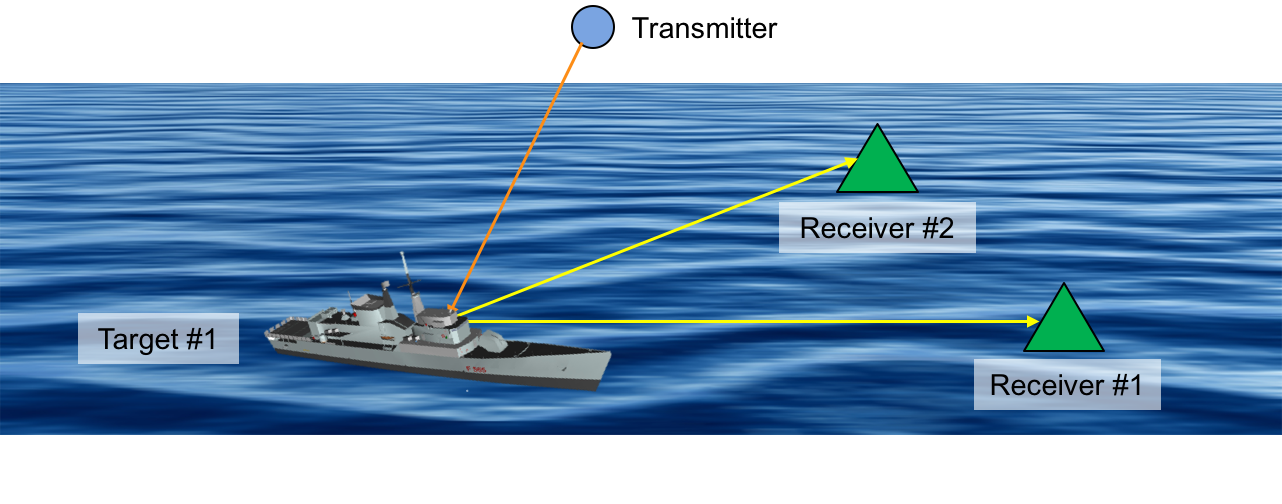
\includegraphics[width=5in]{../media/multistatic/ms_rf_concept.png}
  \end{center}
  \renewcommand{\baselinestretch}{1} \small\normalsize
  \begin{quote}
    \caption[Multistatic RF Sensor Networks Concept]{Multistatic RF Sensor Networks Concept\label{ms_fig:1}}
  \end{quote}
\end{figure}
\renewcommand{\baselinestretch}{2} \small\normalsize

\section{Sources of Uncertainty}
There are 3 primary sources for randomness in propagating through a maritime environment: the configuration of the target ship, the refractivity of the atmosphere, and the sea surface.

The configuration of the target ship drives the RADAR Cross Section (RCS). As shown in Figure \ref{rmt_fig:1}, the RCS signature is complicated and highly aspect dependent. 
\begin{figure}[H]
  \begin{center}
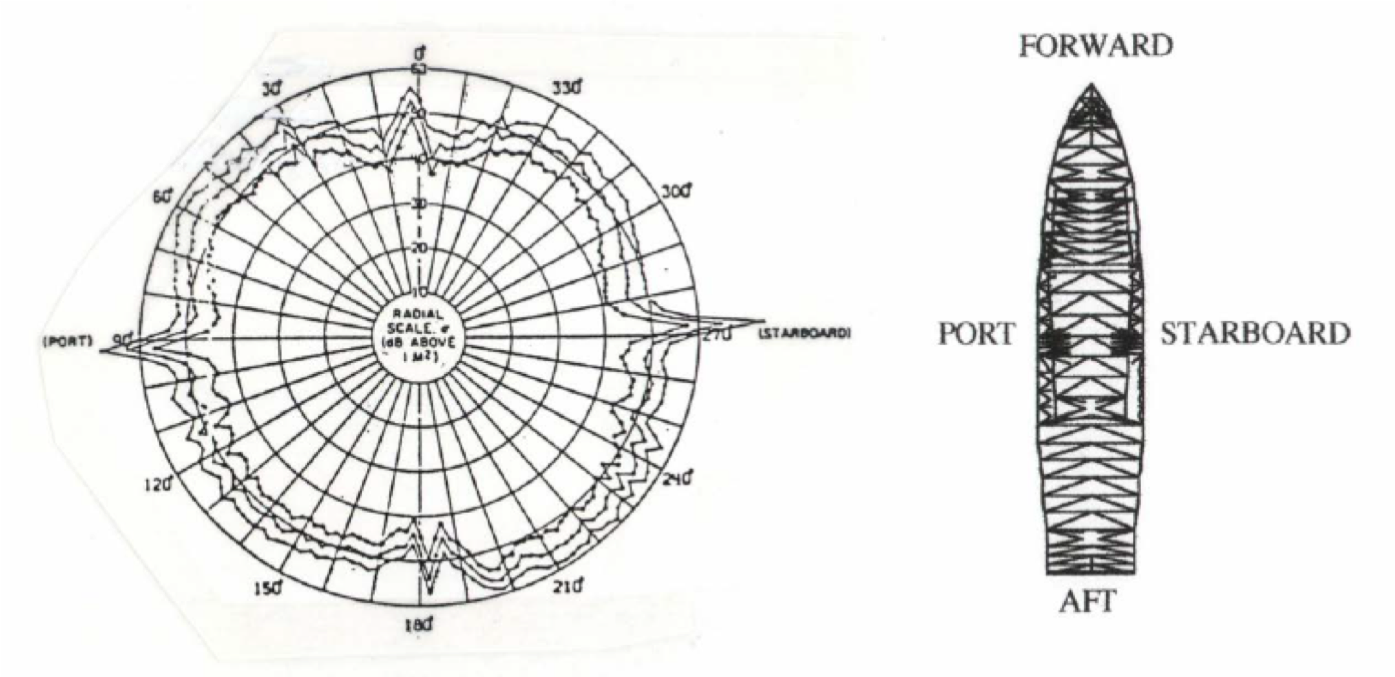
\includegraphics[width=4in]{../media/multistatic/shipconfig.png}
  \end{center}
  \renewcommand{\baselinestretch}{1} \small\normalsize
  \begin{quote}
    \caption[Ship Configuration RCS]{Ship Configuration RCS\label{rmt_fig:1}}
  \end{quote}
\end{figure}
\renewcommand{\baselinestretch}{2} \small\normalsize
The RCS is also impacted by how the specific ship is configured; what it has or doesn't have and how components are arranged on the deck. There are many programs applying significant effort into modeling the behavior of ship RCS signatures, so RCS fluctuations will be considered out of scope for the purposes of this work.

The next source of uncertainty is the refractive index profile of the atmosphere, which can vary significantly as described in Chapter \ref{chapter_env}. As shown in Figure \ref{rmt_fig:2}, a transmitted ray will refract in the atmosphere and follow a curved path. If we use a 4/3 earth model, we can approximate the propagation path as linear and simplify calculations. This approximation no longer holds in the presence of a duct, where the atmosphere acts as a waveguide and extends propagation beyond the horizon, providing a different curve for the ray trajectory.
\begin{figure}[H]
  \begin{center}
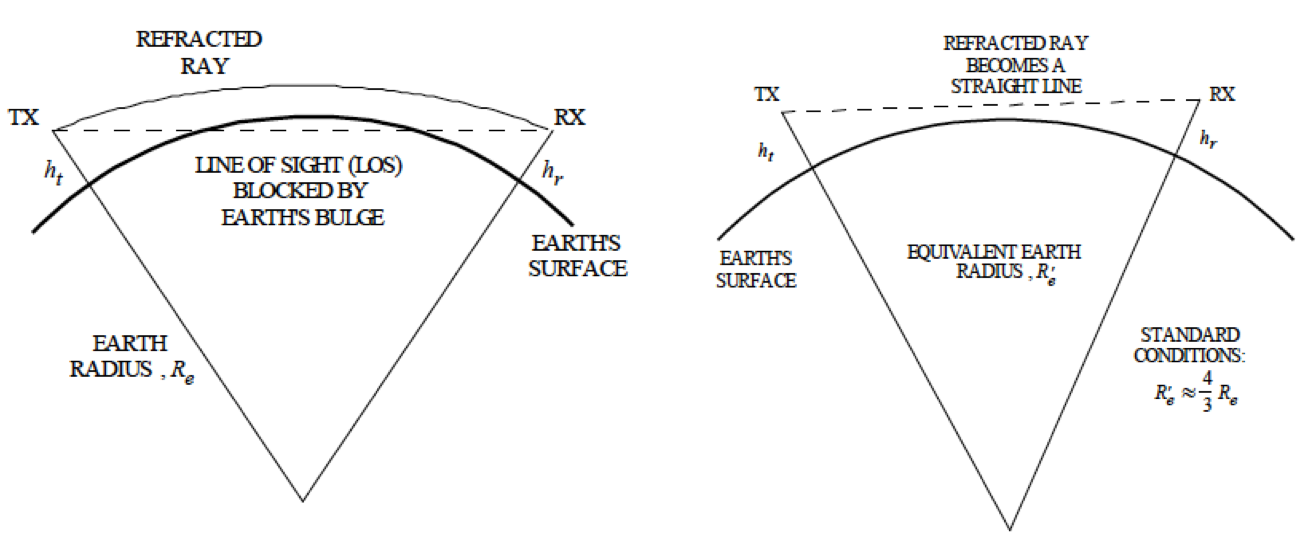
\includegraphics[width=4in]{../media/multistatic/earth_refractivity.png}
  \end{center}
  \renewcommand{\baselinestretch}{1} \small\normalsize
  \begin{quote}
    \caption[4/3 Earth Model and Rectilinear Propagation]{4/3 Earth Model and Rectilinear Propagation\label{rmt_fig:2}}
  \end{quote}
\end{figure}
\renewcommand{\baselinestretch}{2} \small\normalsize
Large scale variations in refractivity occur on the order of several minutes to hours and will not significantly impact the signal statistics over a few pulses or a Coherent Processing Interval (CPI). We will treat refractive index fluctuations as affecting average signal levels rather than variance.

The final source of uncertainty is variations due to the sea surface, which manifest through multipath and clutter. Multipath is due to interference from forward specular reflections and clutter is due to backscatter from the surface. These will both be described in detail in Chapter \ref{chapter_env} and are the primary sources of randomness to be modeled in this work. 


\renewcommand{\thechapter}{2}
\renewcommand{\baselinestretch}{2} \small\normalsize
\section{Random Matrix Theory Overview}
Eugene Wigner developed RMT to describe the statistics of energy levels of large nuclei. He found that if he replaced the Hamiltonian of the systems with a random matrix, the statistical properties of the eigenvalues were in agreement (provided the random matrix was chosen from an appropriate distribution) \cite{ott_chaos}.

Since then, RMT has become extremely useful in characterizing chaotic systems that are highly sensitive to small changes, such as the propagation of electromagnetic waves in dense scattering environments.

\subsection{Wave Chaotic Systems}
The wave equation is linear, so solutions can not be chaotic. However, in the semi-classical limit where the wavelength is much smaller than the characteristic length scale ($\lambda << L$), these solutions can be described by rays with chaotic trajectories. This is also known as the random plane wave hypothesis where we can treat the chaotic propagation problem as a random superposition of plane waves.

For the purposes of this work, the propagation has Time Reversal Symmetry (TRS), so the probability distribution of the Hamiltonian will be invariant under orthogonal transformations, $P(H) = P(O^THO)$ for any orthogonal matrix $O$ \cite{ott_chaos}. This is referred to as the Gaussian Orthogonal Ensemble (GOE) case. Because the matrix $O$ is orthogonal, the elements of the random matrix will be real, independent, and identically distributed (IID) Gaussian random variables with the standard deviation of the diagonal elements equal to twice the standard deviation of the off-diagonal elements.

A simple method to generate a random matrix, $\textbf{M}$, following a GOE distribution is to first generate a matrix, $\textbf{A}$, whose elements are IID zero mean Gaussian random variables with unit standard deviation. The matrix $\textbf{M}$ is then given by

\begin{equation}
\textbf{M} = \frac{1}{2}\left(\textbf{A} + \textbf{A}^T \right)
\label{rmt_eq:000}
\end{equation}
\renewcommand{\baselinestretch}{2} \small\normalsize

Wave chaotic systems have both universal and system specific properties. The system specific features are due to the short orbit trajectories (the paths with few bounces between the ports) and the universal features are due to the chaotic nature of the system itself \cite{bohigas}. RMT works extremely well at predicting the statistical properties of the universal fluctuations; however, short orbit trajectories have a significant impact on the overall scattering statistics and should be included \cite{hart_so} \cite{yeh_universal}. One such model that includes both universal and system specific features is the Random Coupling Model (RCM), which normalizes the impedance matrix by the system specific impedance to separate the universal and system specific features  \cite{zheng_single} \cite{zheng_multiple} \cite{hemmady_review} \cite{gradoni_review}.

One of the primary contributions of the RCM is that it allows the overlap integral which describes the interaction between the eigenmodes and current shape profile to be represented through the radiation impedance of an antenna coupled to the port \cite{hart_time_domain} \cite{zheng_single}.

\subsection{Multi-static Configuration}
The scattering matrix, $\textbf{S}$, contains all the information for the various propagation paths through the system with each transmitter and receiver considered as a port. This matrix then determines the relationship between the output voltages, $\textbf{V}^o$, and the input voltages, $\textbf{V}^i$ \cite{pozar_microwave}.

\begin{equation}
\textbf{V}^o = \textbf{S} \textbf{V}^i
\label{rmt_eq:0}
\end{equation}
\renewcommand{\baselinestretch}{2} \small\normalsize

The scattering matrix is traditionally used in the analysis of transmission lines for microwave engineering, but we can generalize it to a multi-static RF sensor network by considering the columns of $\textbf{S}$ as transmitters and the rows as receivers.
\[\textbf{S}=
\begin{tikzpicture}[baseline=-\the\dimexpr\fontdimen22\textfont2\relax ]

\matrix (m)[matrix of math nodes,left delimiter=(,right delimiter=)]
{
S_{11} & S_{12} & \dots & S_{1n}\\
S_{21} & S_{22} & \dots & S_{2n}\\
\vdots & \vdots & \ddots & \vdots\\
S_{n1} & S_{n2} & \dots & S_{nn}\\
};

\equation (e)[]{};
\begin{pgfonlayer}{myback}
\fhighlight[blue!20]{m-1-1}{m-4-1}
\end{pgfonlayer}
\label{rmt_eq:1}
\end{tikzpicture}
\]
\renewcommand{\baselinestretch}{2} \small\normalsize

For a single transmitter, only the 1st column of $\textbf{S}$ is necessary to describe the statistics. The additional columns can be used to inject disturbance signals such as jamming or other undesired RF noise sources. 

The individual elements of $\textbf{S}$ can be expressed through the RADAR range equation (derived in Chapter \ref{chapter_radar_basics}) where the complex propagation factor, $F_p$, captures all the environment impacts, both configuration dependent and chaotic.
\begin{equation}
S_{n1} = \sqrt{\left|\frac{P_tG_tG_{rn}\lambda^2\sigma_{Bn}F_{p1}F_{pn}}{(4\pi)^3R_1^2R_n^2} \right|}
\label{rmt_eq:2}
\end{equation}
\renewcommand{\baselinestretch}{2} \small\normalsize

The scattering matrix approach captures the universal fluctuations from the underlying chaotic scattering system very well. In the real world, we interact with the chaotic scattering systems through deterministic components (antennas, transmission lines, etc.) that may not be well coupled to the chaotic system. In this case, the scattering matrix does not give us a clean method of separating the random and deterministic parts. To counter this, we can utilize a model such as the RCM and transform the scattering matrix to the impedance matrix, $\textbf{Z}$. The impedance matrix relates the output currents to the input voltages \cite{yeh_first_principles} and naturally separates the random and deterministic components \cite{zheng_single}. 
\begin{equation}
\textbf{Z} = \textbf{Z}_o(1+\textbf{S})(1-\textbf{S})^{-1}
\label{rmt_eq:3}
\end{equation}
\renewcommand{\baselinestretch}{2} \small\normalsize
Here $\textbf{Z}_o$ is a diagonal matrix that captures the characteristic impedance of transmission lines connected to the ports.

\renewcommand{\thechapter}{3}
\chapter{RADAR Basics}\label{chapter_radar_basics}
This chapter covers some RADAR basics, including the RADAR range equation, propagation factors, and bistatic configurations.

\section{RADAR Range Equation} 
The RADAR range equation provides a deterministic method to calculate received signal levels and is the workhorse for analyzing RADAR system performance. This equation is the first step towards building a statistical model, as it captures the underlying physics.

\subsection{Monostatic Case}
The RADAR range equation is derived by assuming spherically propagating waves and computing the propagated power at 4 incremental points between the transmitter and target as shown in Figure \ref{intro_fig:1}. These points are the projected power ($P_1$), the power received at the target ($P_2$), the power reflected by the target ($P_3$), and the power at the receiver antenna ($P_4$). The received power ($P_r$) is then the product of $P_4$ and the effective area of the receiver antenna.

\begin{figure}[H]
  \begin{center}
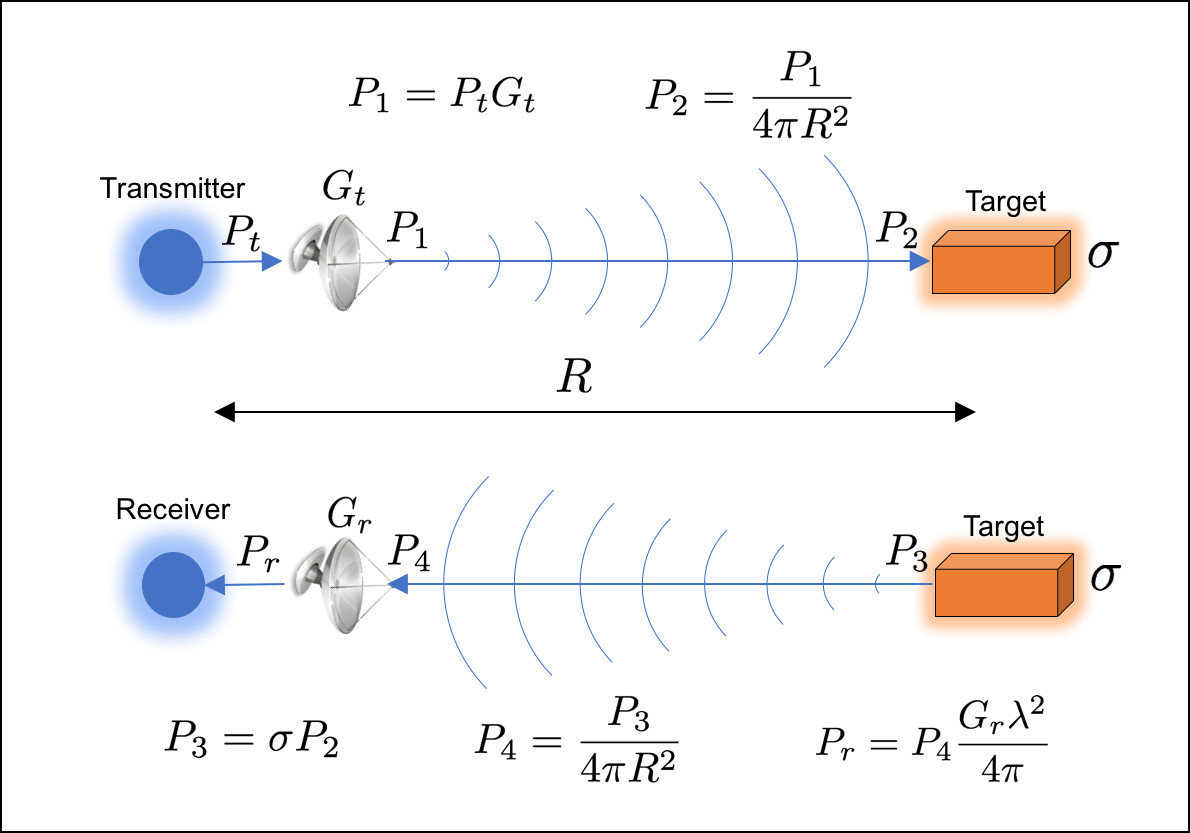
\includegraphics[width=4in]{../media/multistatic/radar_range_equation.png}
  \end{center}
  \renewcommand{\baselinestretch}{1} \small\normalsize
  \begin{quote}
    \caption[RADAR Range Equation Derivation]{RADAR Range Equation Derivation \label{intro_fig:1}}
  \end{quote}
\end{figure}
\renewcommand{\baselinestretch}{2} \small\normalsize

With spherical waves, the power is spread out over a sphere of radius equal to the slant range, $R$, which gives a scaling factor of $\left( 4\pi R^2 \right)^{-1}$ for propagation. The total projected power, $P_1$, is the transmitted power, $P_t$, multiplied by the antenna gain, $G_t$. The RCS, $\sigma$, defines the amount of power reflected, and the effective area of the antenna is $G_t\lambda^2(4\pi)^{-1}$.

In the monostatic case, $G_t = G_r$ and the RADAR range equation is then \cite{skolnik_handbook}.
  \begin{equation}
  \label{intro_eq:1}
 P_r = \frac{P_tG_t^2\sigma\lambda^2}{\left(4\pi\right)^3R^4}
  \end{equation}
In this equation, the antenna gain, $G_t$ is a function of the angle between the antenna boresight and the target. Randomness enters this version of the RADAR range equation through the target RCS as there is otherwise no term to account for environmental fluctuations.

In the atmosphere, propagation is a linear operation. Therefore we can leverage superposition to compute the RADAR range equation for each path or scatterer and sum the results.

We can divide Equation \ref{intro_eq:1} by the noise power to represent the RADAR range equation in terms of signal to noise ratio (SNR) \cite{skolnik_handbook}.
\begin{equation}
    \label{intro_eq:2}
\text{SNR} = \frac{P_r}{P_n} = \frac{P_tG_t^2\sigma\lambda^2}{\left(4\pi\right)^3 R^4k_BTBF_n}
\end{equation}
In this equation, $k_B$ is the Boltzmann constant, $B$ is the receiver bandwidth, $T$ is the receiver temperature and $F_n$ is the receiver noise figure. Nominally, $B$ is taken to be the inverse of the pulse width to accomodate matched filter processing and $T$ is taken to be $300$ K.

\subsection{Bistatic Case}
In the bistatic case, we need to consider each path separately as the ranges, antenna gains, and RCS are all likely different. The standard bistatic RADAR range equation is shown in Equation \ref{intro_eq:3}.
  \begin{equation}
  \label{intro_eq:3}
 P_r = \frac{P_tG_tG_r\sigma_B\lambda^2}{\left(4\pi\right)^3R_1^2R_2^2}
  \end{equation}
In this equation, $G_t$ is the antenna gain for the transmitter, $G_r$ is the antenna gain for the receiver, $\sigma_B$ is the bistatic RCS, $R_1$ is the slant range along the first path (transmitter to target), and $R_2$ is the slant range along the second path (target to receiver). Again, the antenna gains, $G_t$ and $G_r$ are functions of the angle between the antenna boresight and the target.

The bistatic RADAR range equation in terms of SNR is shown in Equation \ref{intro_eq:4}.
\begin{equation}
    \label{intro_eq:4}
\text{SNR} = \frac{P_tG_tG_r\sigma_B\lambda^2}{\left(4\pi\right)^3 R_1^2R_2^2k_BTBF_n}
\end{equation}

\subsection{Propagation Factors}
The use of a propagation factor, $F_p$, allows us to include atmospheric effects in the RADAR range equation. These effects can include absorption from atmospheric gases and weather such as rain or snow as well as rollups for the effects of multipath reflections, diffraction from the surface, and clipping by the horizon. The propagation factor is typically implemented as a multiplier to the RADAR range equation and provides another mechanism to introduce randomness. Because they encompasses a wide variety of environment conditions, propagation factors are generally complicated to compute. 

The bistatic RADAR range equation with a propagation factor included is given in Equation \ref{intro_eq:4a}.
  \begin{equation}
  \label{intro_eq:4a}
 P_r = \frac{P_tG_tG_r\sigma_B\lambda^2}{\left(4\pi\right)^3R_1^2R_2^2}F_p
  \end{equation}
  
To visualize the propagation factors, Figure \ref{intro_fig:1a} shows the propagation factors for standard atmosphere and Figure \ref{intro_fig:1b} shows the propagation factors with a 20 m duct. With standard atmosphere, we can see the impact of the horizon as well as the periodic multipath peaks and nulls. With a 20 m duct, the atmosphere acts as a waveguide (described in detail in Chapter \ref{chapter_env}) so that propagation extends past the horizon.
  \begin{figure}[H]
  \begin{center}
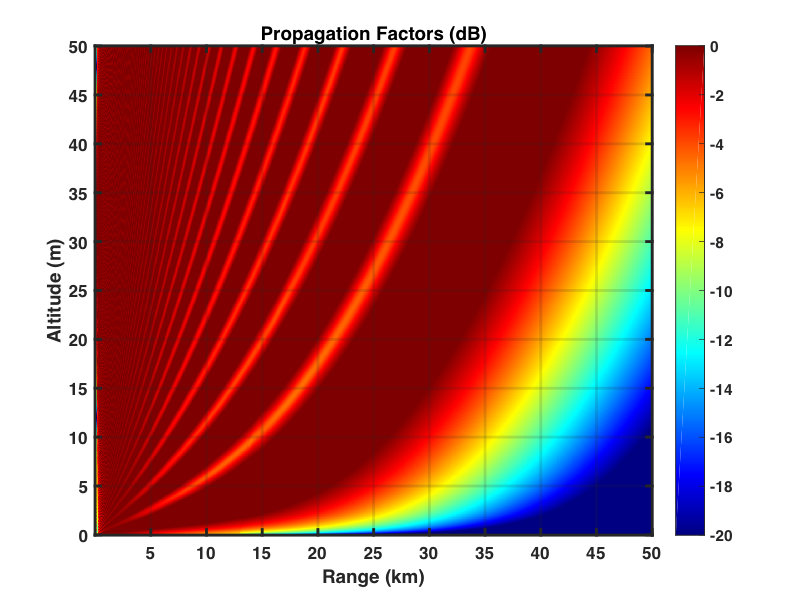
\includegraphics[width=4in]{../media/multistatic/std_atmos_pf.png}
  \end{center}
  \renewcommand{\baselinestretch}{1} \small\normalsize
  \begin{quote}
    \caption[Propagation Factors for Standard Atmosphere]{Propagation Factors for Standard Atmosphere \label{intro_fig:1a}}
  \end{quote}
\end{figure}
\renewcommand{\baselinestretch}{2} \small\normalsize

\begin{figure}[H]
  \begin{center}
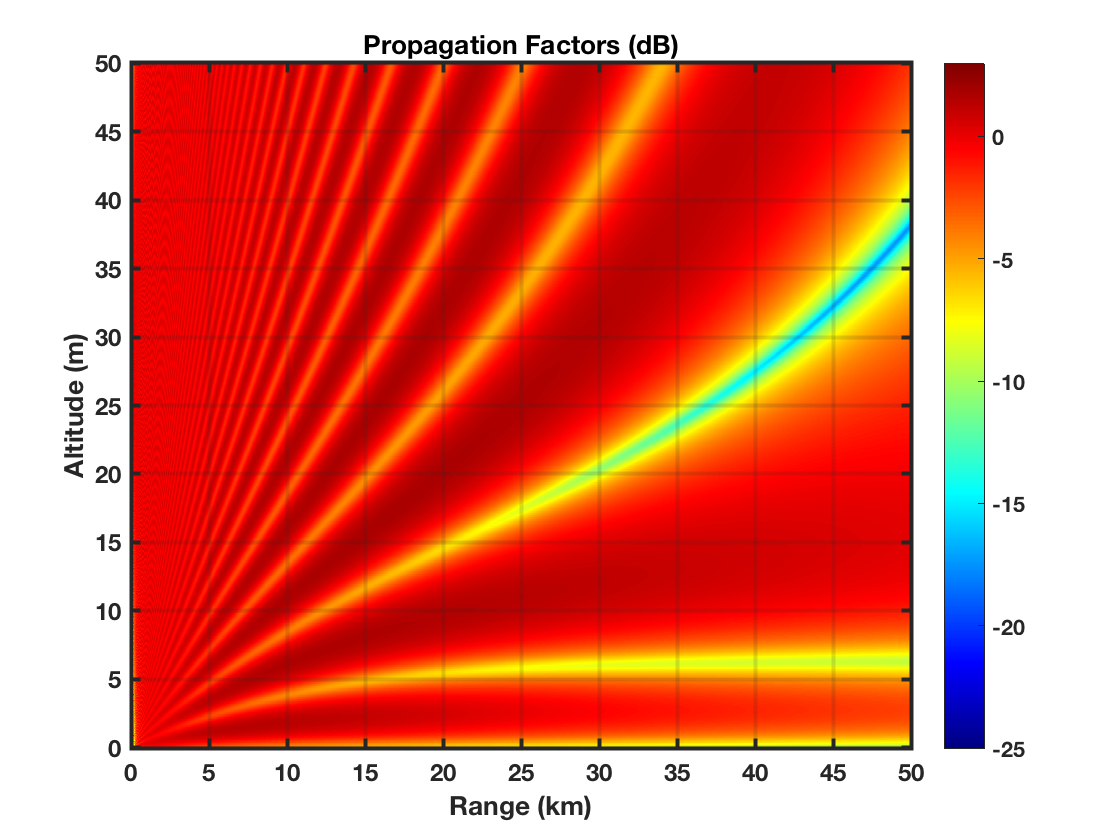
\includegraphics[width=4in]{../media/multistatic/20m_duct_pf.png}
  \end{center}
  \renewcommand{\baselinestretch}{1} \small\normalsize
  \begin{quote}
    \caption[Propagation Factors for a 20 m Duct]{Propagation Factors for a 20 m Duct \label{intro_fig:1b}}
  \end{quote}
\end{figure}
\renewcommand{\baselinestretch}{2} \small\normalsize

\section{Bistatic Configurations}
Because the transmitter and receiver are not colocated in a bistatic configuration, the geometry now becomes ellipsoidal as shown in Figure \ref{intro_fig:2}. Here, $R_1$ is the slant range from the transmitter to the target, $R_2$ is the slant range from the target to the receiver, $\theta_t$ is the one way beam width of the transmitter and $\theta_r$ is the one way beam width of the receiver. The bistatic angle, $\beta$, is the angle between the transmitter and receiver in the plane containing the transmitter, receiver, and target. 
\begin{figure}[H]
  \begin{center}
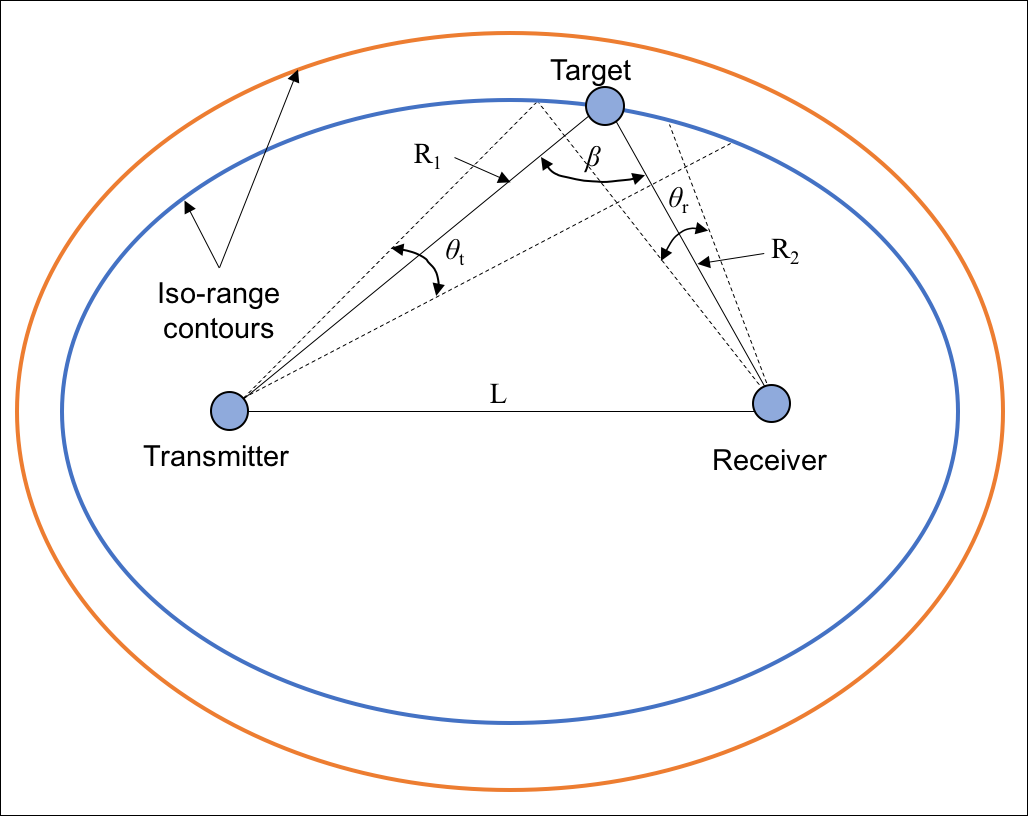
\includegraphics[width=4in]{../media/multistatic/Isorange_contours.png}
  \end{center}
  \renewcommand{\baselinestretch}{1} \small\normalsize
  \begin{quote}
    \caption[Isorange Contours for Bistatic Configuration]{Isorange Contours for Bistatic Configuration \label{intro_fig:2}}
  \end{quote}
\end{figure}
\renewcommand{\baselinestretch}{2} \small\normalsize
The isorange contours are defined as the curves where the total path length, $R_1 + R_2$, is constant . These contours form ellipses with the transmitter and receiver at the foci as shown in the blue and orange curves in Figure \ref{intro_fig:2}. For the monostatic case, the isorange contours are simply circles and the geometry is simplified as everything is symmetric. In the bistatic case, however, the beam width is not symmetric along the isorange contours, which results in skewing the impact of clutter.

It is often convenient to look at things in terms of SNR. In a bistatic configuration, the loci of constant SNR are known as the ovals of Cassini \cite{willis_bistatic} and an example is shown in Figure \ref{intro_fig:3}.
\begin{figure}[H]
  \begin{center}
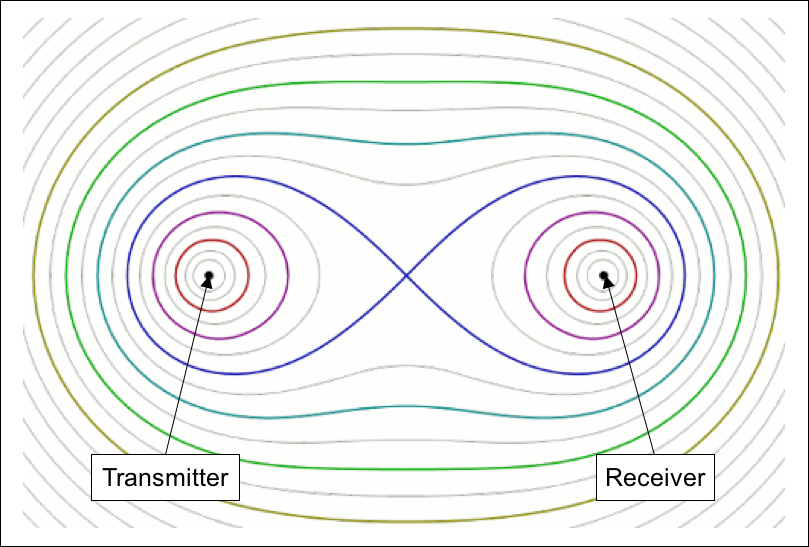
\includegraphics[width=4in]{../media/multistatic/ovals_of_cassini.png}
  \end{center}
  \renewcommand{\baselinestretch}{1} \small\normalsize
  \begin{quote}
    \caption[Ovals of Cassini]{Ovals of Cassini\label{intro_fig:3}}
  \end{quote}
\end{figure}
\renewcommand{\baselinestretch}{2} \small\normalsize
The ovals of Cassini are a simplification that assumes the target RCS and propagation factors are invariant with respect to angle and range. This is rarely the case, but the ovals of Cassini are useful to quickly represent system constraints.

For large SNR, the ovals of Cassini collapse around the transmitter and receiver and define the transmitter centered and receiver centered regions. The cosite region is defined as when the ovals of Cassini surround both the transmitter and receiver \cite {willis_bistatic}.

\renewcommand{\thechapter}{4}
\renewcommand{\baselinestretch}{2} \small\normalsize
\chapter{Environmental Impacts on Electromagnetic Wave Propagation}
Before developing a statistical model, we need to understand which environmental factors affect propagation. Multipath, clutter, and sea spikes are all induced by reflections from the sea surface while changes in the index of refraction cause electromagnetic waves to bend. We will first describe the various earth models that are used along with the propagation geometry that follows from these models. Next we will discuss refractivity and anomalous propagation before covering the reflective effects of multipath, clutter, and sea spikes. We will close this chapter with a discussion of the RCS of targets.

\section{Earth Models}
The earth can be modeled as flat to simplify calculations, as a sphere to capture horizon effects for long range propagation, or as an ellipsoid to provide additional geometric accuracy. In general, the standard model is spherical with the 4/3 earth radius approximation.

\subsection{Flat Earth}
The flat earth model is valid only for short ranges as there is no concept of the RADAR horizon. The geometry provides a simple planar surface such that the local tangent plane is equivalent at both the transmitter and target. This model is shown in Figure \ref{env_fig:1}, where $h$ is the altitude of the transmitter, $h_t$ is the altitude of the target, $R$ is the slant range, $\alpha$ is the depression angle, and $\chi$ is the grazing angle. Also shown in this figure is a single multipath bounce off the surface (the direct path between the transmitter and receiver is not shown). 

\begin{figure}[H]
  \begin{center}
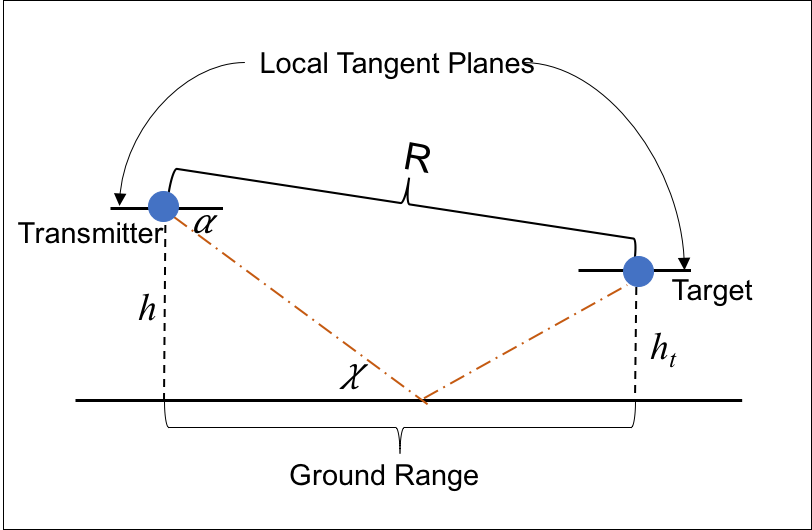
\includegraphics[width=4in]{../media/multistatic/flat_earth_geometry.png}
  \end{center}
  \renewcommand{\baselinestretch}{1} \small\normalsize
  \begin{quote}
    \caption[Flat Earth Geometry]{Flat Earth Geometry\label{env_fig:1}}
  \end{quote}
\end{figure}
\renewcommand{\baselinestretch}{2} \small\normalsize
Flat earth approximations are typically used for initial back of the envelope calculations but should not be used to assess critical performance characteristics. 

\subsection{Spherical Earth}
The spherical earth model assumes the earth is a sphere, with a constant radius $r_e = 6370$ km and is shown in Figure \ref{env_fig:2}. In this figure, $r_e'$ represents the effective radius of the earth.

\begin{figure}[H]
  \begin{center}
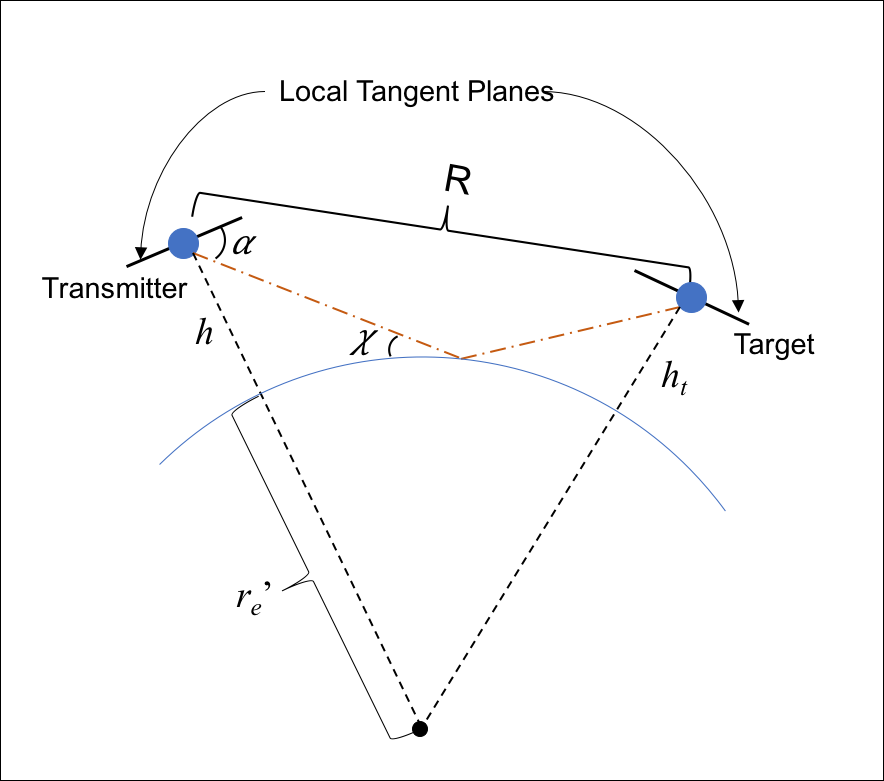
\includegraphics[width=4in]{../media/multistatic/spherical_earth_geometry.png}
  \end{center}
  \renewcommand{\baselinestretch}{1} \small\normalsize
  \begin{quote}
    \caption[Spherical Earth Geometry]{Spherical Earth Geometry\label{env_fig:2}}
  \end{quote}
\end{figure}
\renewcommand{\baselinestretch}{2} \small\normalsize
The curvature of the earth changes the reference planes between the transmitter and target, so that the local tangent planes are not equivalent.

\subsection{WGS-84 Earth}
The World Geodetic System (WGS) is an earth fixed standard coordinate system developed in 1984 and the current standard is identified as WGS-84 \cite{dod_wgs84}. This model is not generally used for RADAR calculations as it complicates analysis beyond the spherical earth model and the difference between the two models is negligible compared to the uncertainty in the refractive index profile. In cases where we desire the additional geometry accuracy, such as RADAR horizon calculations at a particular location on the earth, we can follow the spherical earth model but use the local radius of curvature from the WGS-84 earth model as $r_e$.

\subsection{4/3 Earth Model}
Due to the refractive index of the atmosphere, the propagation path of an electromagnetic wave will curve. Under the assumption of standard atmospheric conditions, the propagation path can be approximated as a straight line if an effective radius of the earth is used, $r_e' = 4/3 r_e$ \cite{blake_radar}, \cite{nathanson_radar}. This is referred to as the 4/3 earth model and is used in most analytical calculations.

As stated above, we can increase geometric accuracy for locality by using the local radius of curvature from the WGS-84 model for $r_e$.

\section{Geometry}
The earth model used defines the propagation geometry. The geometric aspects of most importance are the grazing angle, depression angle, and RADAR horizon. The grazing and depression angles are important in computing the reflection coefficients and beam intersection area for both clutter and multipath and the RADAR horizon bounds the propagation range.

\subsection{Grazing and Depression Angles}
The grazing and depression angles are both defined for rays intersecting the earth as shown in Figure \ref{env_fig:2}. The depression angle, $\alpha$ is the angle from the local horizontal plane at the transmitter and is given by Equation \ref{env_eq:1} \cite{nathanson_radar}.
\begin{equation}
  \label{env_eq:1}
  \alpha = \sin^{-1}\left(\frac{2r_e'h + h^2 + R^2}{2R\left[r_e' + h \right]} \right)
  \end{equation}
  
The grazing angle, $\chi$, is the angle from the local horizontal plane at the target and is given by Equation \ref{env_eq:2} \cite{nathanson_radar}.
  \begin{equation}
  \label{env_eq:2}
  \chi = \sin^{-1}\left(\frac{h}{R}\left[1 + \frac{h}{2r_e'} \right] - \frac{R}{2r_e'} \right)
  \end{equation}
  
In the flat earth case, the grazing and depression angles are equal. The curvature of the earth changes the local tangent plane reference, so they are not equal in the case of a spherical or ellipsoidal earth.
  
\subsection{RADAR Horizon}
The curvature of the earth puts an upper limit on the distance an electromagnetic wave can travel before intercepting the earth. The range to the horizon, $R_h$, is given by Equation \ref{env_eq:3}. Slant ranges greater than this distance will be clipped by the earth and not reach the target unless anomalous propagation conditions (ducting) are present.
  \begin{equation}
  \label{env_eq:3}
  R_h = \sqrt{2r_e'h + h^2} + \sqrt{2r_e'h_t + h_t^2}
  \end{equation}
In this equation, $h$ is the altitude of the transmitter and $h_t$ is the altitude of the target.

Because an electromagnetic wave consists of a finite bundle of rays rather than a single ray, the physical clipping by the horizon is gradual rather than instantaneous. The impact of the horizon should be modeled by a smooth rolloff rather than a step function.
  
\section{Atmospheric Refraction Effects}
\subsection{Refractivity}\label{env_sec:refractivity}

\subsection{Ducting}

\section{Multipath}
Multipath refers to reflections from the surface of the earth resulting in many paths between the transmitter and the target. When these paths are in phase, the signal at the target is amplified. When these paths are out of phase, the signal is reduced and referred to as a multipath null.

\subsection{2-Ray Model}
The 2-Ray Model for multipath is shown in Figure \ref{env_fig:3}, using a flat earth geometry to simplify the explanation. In this model, the two rays are the direct path from the transmitter to the target and a single multipath bounce from the surface between the transmitter and target.
\begin{figure}[H]
  \begin{center}
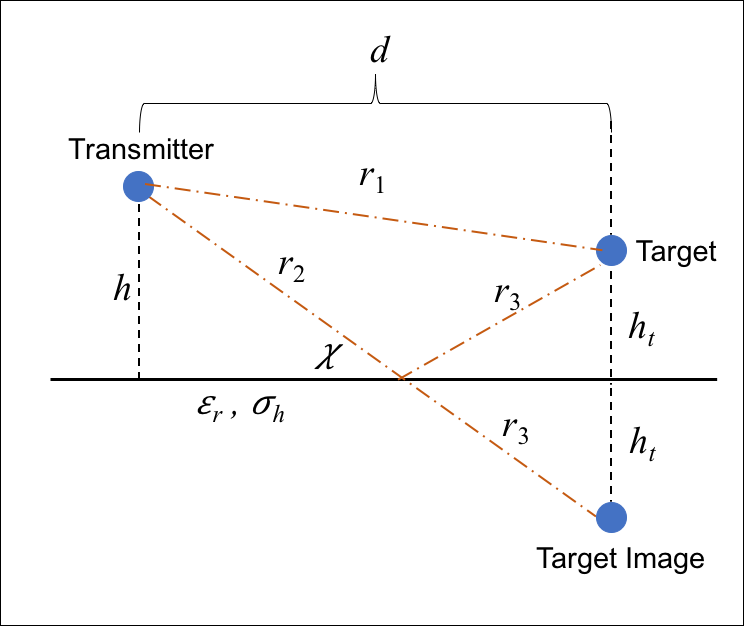
\includegraphics[width=4in]{../media/multistatic/two_ray_multipath_model.png}
  \end{center}
  \renewcommand{\baselinestretch}{1} \small\normalsize
  \begin{quote}
    \caption[Two Ray Multipath Model]{Two Ray Multipath Model\label{env_fig:3}}
  \end{quote}
\end{figure}
\renewcommand{\baselinestretch}{2} \small\normalsize
The sea surface is characterized by its dielectric constant, $\epsilon_r$ and the height variance, $\sigma_h$, which will result in a reflection coefficient, $\Gamma_t$. We can characterize the multipath ray by using the image of the target.

Following \cite{lohrmann_rcs}, we can use superposition and express the combination of the rays as a propagation factor, $F_p$:
  \begin{equation}
  \label{env_eq:3b}
F_p = e^{jkr_1} + \Gamma_te^{jk\left(r_2 + r_3\right)}
\end{equation}

In both expressions, the result is dependent on the phase difference between the path distances $r_1$ and $r_2 + r_3$. This means we will have a multipath null (destructive interference) whenever $k\left(r_1 + r_2 + r_3\right) = (2m + 1)\pi$ and we will have a multipath peak (constructive interference) whenever $k\left(r_1 + r_2 + r_3\right) = 2m\pi$. From geometry, we can see that $r_1 = \sqrt{d^2 + (h-h_t)^2}$ and $r_2 + r_3 = \sqrt{d^2 + (h+h_t)^2}$

Figure \ref{env_fig:3t} shows an example of the propagation factor from the two ray multipath model with $h = 15m$, $h_t = 15m$, $f = 35GHz$, and $\Gamma_t = 1$. 
\begin{figure}[H]
  \begin{center}
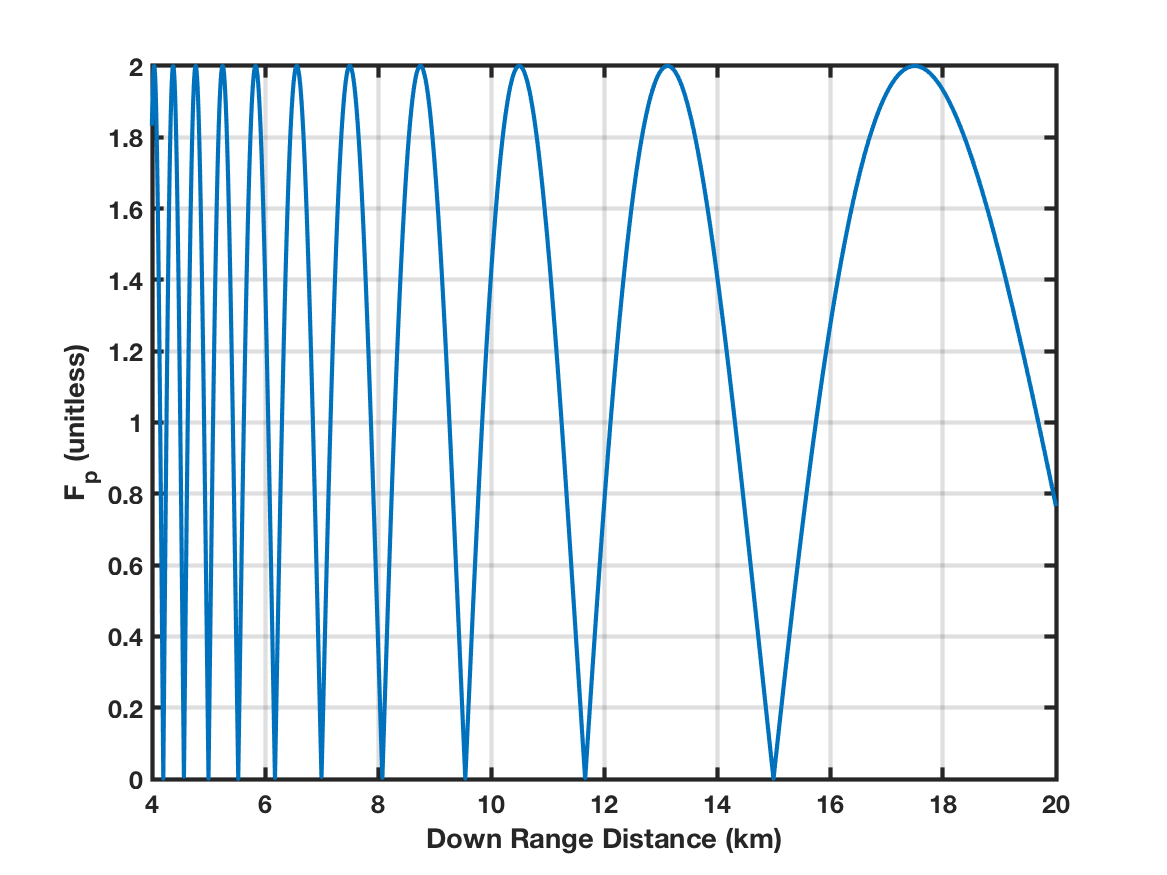
\includegraphics[width=4in]{../media/multistatic/two_ray_multipath_results.png}
  \end{center}
  \renewcommand{\baselinestretch}{1} \small\normalsize
  \begin{quote}
    \caption[Two Ray Multipath Model Results]{Two Ray Multipath Model Results\label{env_fig:3t}}
  \end{quote}
\end{figure}
\renewcommand{\baselinestretch}{2} \small\normalsize


\subsection{Reflection Coefficient}
From \cite{miller_reflection}, we can express the rough sea surface reflection coefficient, $\rho$, by Equation \ref{env_eq:4}. 
  \begin{equation}
  \label{env_eq:4}
\rho = \left|\frac{\bar{E}}{E_\delta \Gamma} \right| = e^{-2\left[2\pi g \right]^2}I_0\left( 2\left[2\pi g \right]^2\right) 
\end{equation}
In this equation, $g = \sigma_h\sin(\chi)/\lambda$, $\bar{E}$ is the average electric field reflected from the surface, $E_\delta$ is the incident electric field, $\Gamma$ is the smooth (Fresnel) reflection coefficient, and $I_0$ is the modified Bessel function of the first kind.

The smooth reflection coefficient depends on the polarization of the incident wave and is given by Equation \ref{env_eq:5} for horizontal polarization and by Equation \ref{env_eq:6} for vertical polarization.
  \begin{equation}
  \label{env_eq:5}
 \Gamma_h = \frac{\sin(\chi)- \sqrt{\epsilon_r - \cos^2(\chi)}}{\sin(\chi) + \sqrt{\epsilon_r - \cos^2(\chi)}}
  \end{equation}
  
  \begin{equation}
  \label{env_eq:6}
 \Gamma_v = \frac{\sin(\chi)- \sqrt{\frac{\epsilon_r - \cos^2(\chi)}{\epsilon_r^2}}}{\sin(\chi) + \sqrt{\frac{\epsilon_r - \cos^2(\chi)}{\epsilon_r^2}}}
  \end{equation}
In these equations, $\epsilon_r$ is the relative permittivity of the ocean and is given by Equation \ref{env_eq:7} at $20^{\circ}$ C and $3.6\%$ salinity for an electromagnetic wave with temporal frequency $f$. 
  
\begin{equation}
  \label{env_eq:7}
\epsilon_r = \left[\frac{64.18}{1 + 3.30523\times 10^{-21}f^2} + 4.9 \right] + j\left[\frac{3.689792\times 10^{-9}f}{1 + 3.30523\times 10^{-21}f^2} + \frac{9.4\times 10^{10}}{f} \right]
  \end{equation}
  
The total reflection coefficient, $\Gamma_t$ is then the product of the rough and smooth reflection coefficients, $\Gamma_t = \rho\Gamma_h$ or $\Gamma_t = \rho\Gamma_v$.

\section{Clutter}
\subsection{Beam Limited Case}
\subsection{Pulse Limited Case}
\subsection{Backscatter Coefficient}

\section{SeaSpikes}

\section{Target RCS}
\subsection{Point Targets}
\subsection{Complex Targets}
\subsection{Fluctuating Target Models}
For traditional monostatic RADAR systems, work done by Jess Marcum and Peter Swerling provided statistical models for the RCS of targets in the ocean\cite{richards_radar}. There are $4$ Swerling cases that are generally considered, using $2$ different decorrelation time lengths and $2$ different PDFs as shown in Table \ref{env_tab:1}. 

\begin{table}[H]
  \begin{center}
      \renewcommand{\baselinestretch}{1} \small\normalsize
  \begin{quote}
    \caption[Swerling Fluctuating Target RCS Model Description]{Swerling Fluctuating Target RCS Model Description\label{env_tab:1}}
  \end{quote}
  \begin{tabular} {|c | c | c |}
    \hline
  \bf{Case} & \bf{Decorrelation Time Length} & \bf{Chi-squared PDF Degree} \\ \hline
  1 &Long (Scan to Scan) &2 \\ \hline
  2 &Short (Pulse to Pulse) &2 \\ \hline
  3 &Long (Scan to Scan) &4 \\ \hline
  4 &Short (Pulse to Pulse) &4 \\ \hline
\end{tabular}
\end{center}
\end{table}
\renewcommand{\baselinestretch}{2} \small\normalsize
The Chi-squared PDF of degree $2$ covers the case with many randomly distributed small scatterers with none dominant and the Chi-squared PDF of degree $4$ covers the case with a single dominant scatterer and many small scatterers. These PDFs are shown in Figure \ref{env_fig:3}.
\begin{figure}[H]
  \begin{center}
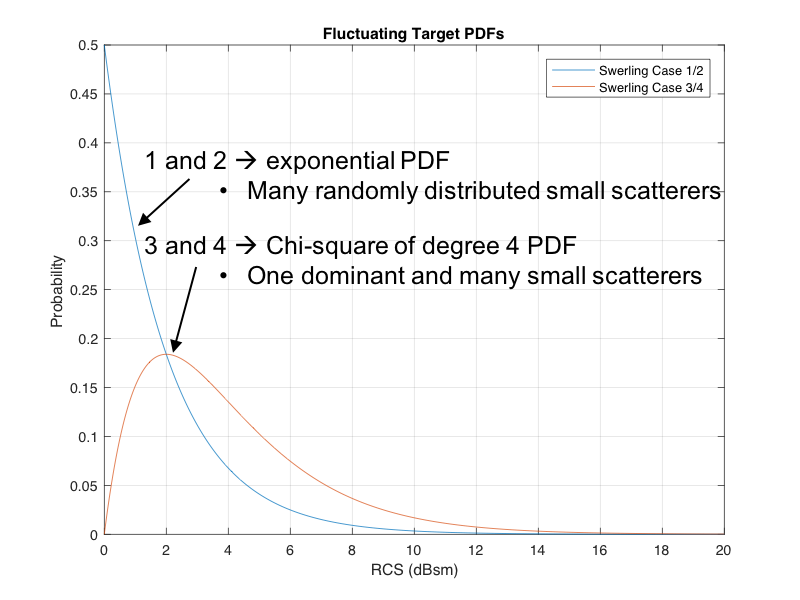
\includegraphics[width=4in]{../media/multistatic/swerling_pdfs.png}
  \end{center}
  \renewcommand{\baselinestretch}{1} \small\normalsize
  \begin{quote}
    \caption[Swerling Target Fluctuation Model PDFs]{Swerling Target Fluctuation Model PDFs\label{env_fig:3}}
  \end{quote}
\end{figure}
\renewcommand{\baselinestretch}{2} \small\normalsize

The long decorrelation time covers the case where the target RCS can be considered constant over the time the RADAR performs a single scan and the short decorrelation time covers the case where the target RCS changes on a pulse to pulse basis. Modern RADAR systems operate in frequency agile modes where the carrier frequency is changed each pulse, in which case the decorrelation time can be considered to be short. A fluctuating signal can have a significant effect on $P_d$, as seen in Figure \ref{env_fig:4} which shows $P_d$ as a function of SNR for the nonfluctating case and each of the $4$ Swerling cases. In this figure, we can see that using the wrong PDF can result in significantly overestimating $P_d$.
\begin{figure}[H]
  \begin{center}
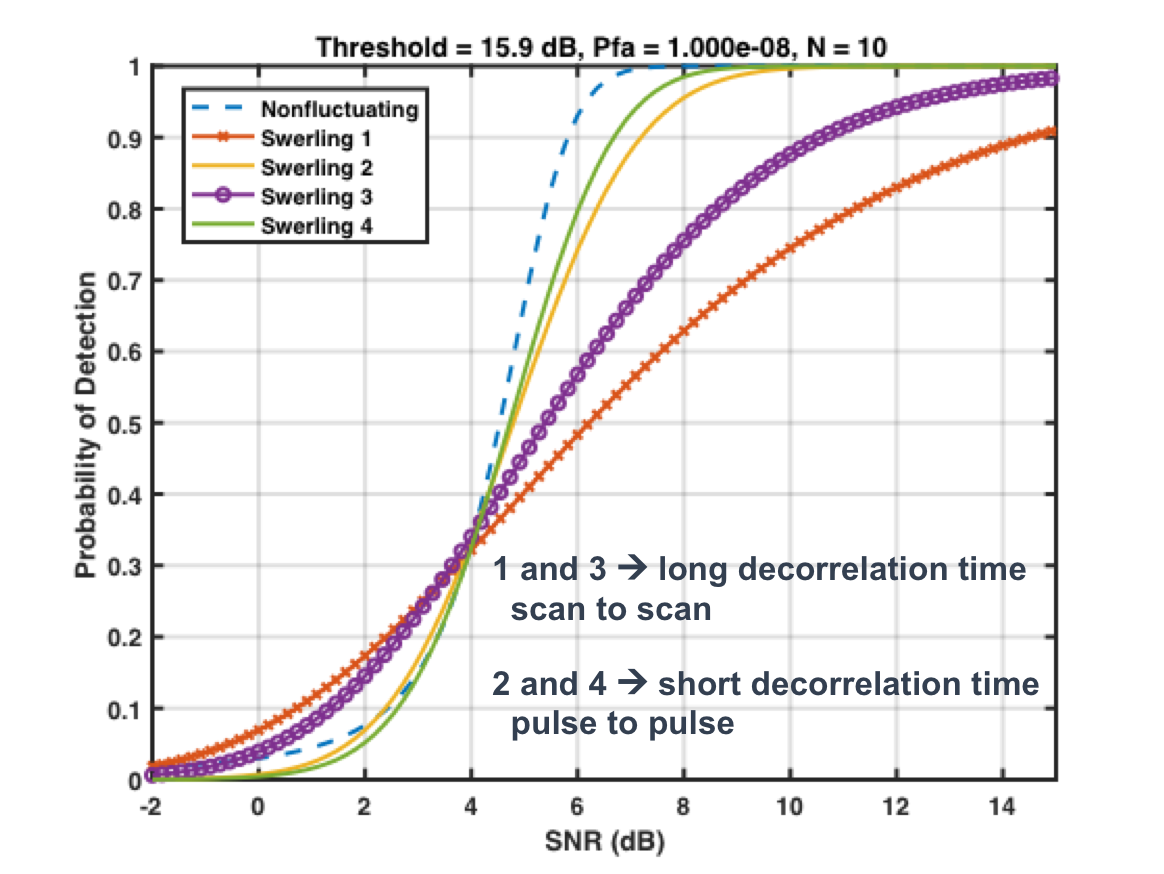
\includegraphics[width=4in]{../media/multistatic/swerling_pd.png}
  \end{center}
  \renewcommand{\baselinestretch}{1} \small\normalsize
  \begin{quote}
    \caption[Swerling Target Fluctuation Model Probability of Detection]{Swerling Target Fluctuation Model Probability of Detection\label{env_fig:4}}
  \end{quote}
\end{figure}
\renewcommand{\baselinestretch}{2} \small\normalsize

Figure \ref{env_fig:4} also shows that $P_d$ is higher with a dominant scatterer than with a collection of uniform scatterers and that it is higher for a short decorrelation time than a long decorrelation time. We can force the decorrelation time to be short by operating in a frequency agile mode, but we generally have no control over the target configuration.

Modeling the RCS for a Swerling fluctuating target is straightforward. We can generate random variables following a Chi-squared distribution of degree $n$ by the sum of $n$ squared normally distributed random variables with zero mean and unit variance. The mean of the Chi-squared distribution is equal to the degree, so to force the mean to a specified deterministic RCS mean, we need to add the deterministic mean and subtract the degree.

Swerling cases 1 and 2 follow a Chi-squared distribution of degree 2. To generate a random variable, $w_{1,2}$, for our RCS, we need to generate 2 normally distributed random variables, $u_1$ and $u_2$. Then, $w_{1,2}$ is given by Equation \ref{env_eq:8}, where $\sigma$ is the deterministic RCS value.
\begin{equation}
  \label{env_eq:8}
w_{1,2} = u_1^2 + u_2^2 + \sigma - 2
  \end{equation}

Swerling cases 3 and 4 follow a Chi-squared distribution of degree 4. To generate a random variable, $w_{3,4}$, for our RCS, we need to generate 4 normally distributed random variables, $u_1$, $u_2$, $u_3$, and $u_4$. Then, $w_{3,4}$ is given by Equation \ref{env_eq:9}, where $\sigma$ is again the deterministic RCS value.
\begin{equation}
  \label{env_eq:9}
w_{3,4} = u_1^2 + u_2^2 + u_3^2 + u_4^2 + \sigma - 4
  \end{equation}
  
The decorrelation time then determines when to perform the random draws; this can be every pulse, every CPI, or at some predetermined time interval. When we have multiple transmitters, we need to be careful about when to schedule the random draws so that one actor does not influence the other.  

\renewcommand{\thechapter}{5}
\chapter{Analytical Propagation}
\label{analytical_propagation}

\section{2-Ray Model}
The 2-Ray multipath model over a flat earth is given in Figure \ref{mp_fig:1}. In this figure, $P_1$ and $P_2$ are the two points we are interested in propagating between and $P_2'$ is the mirror image of $P_2$. $L_1$ is then the direct path and $L_{so}$ represents the shortest orbit reflection from the sea surface. The altitudes of the two points from the mean sea surface are $h_1$ and $h_2$, the total downrange distance is $L$, and the distance to the reflection point is $x_m$.

\begin{figure}[H]
  \begin{center}
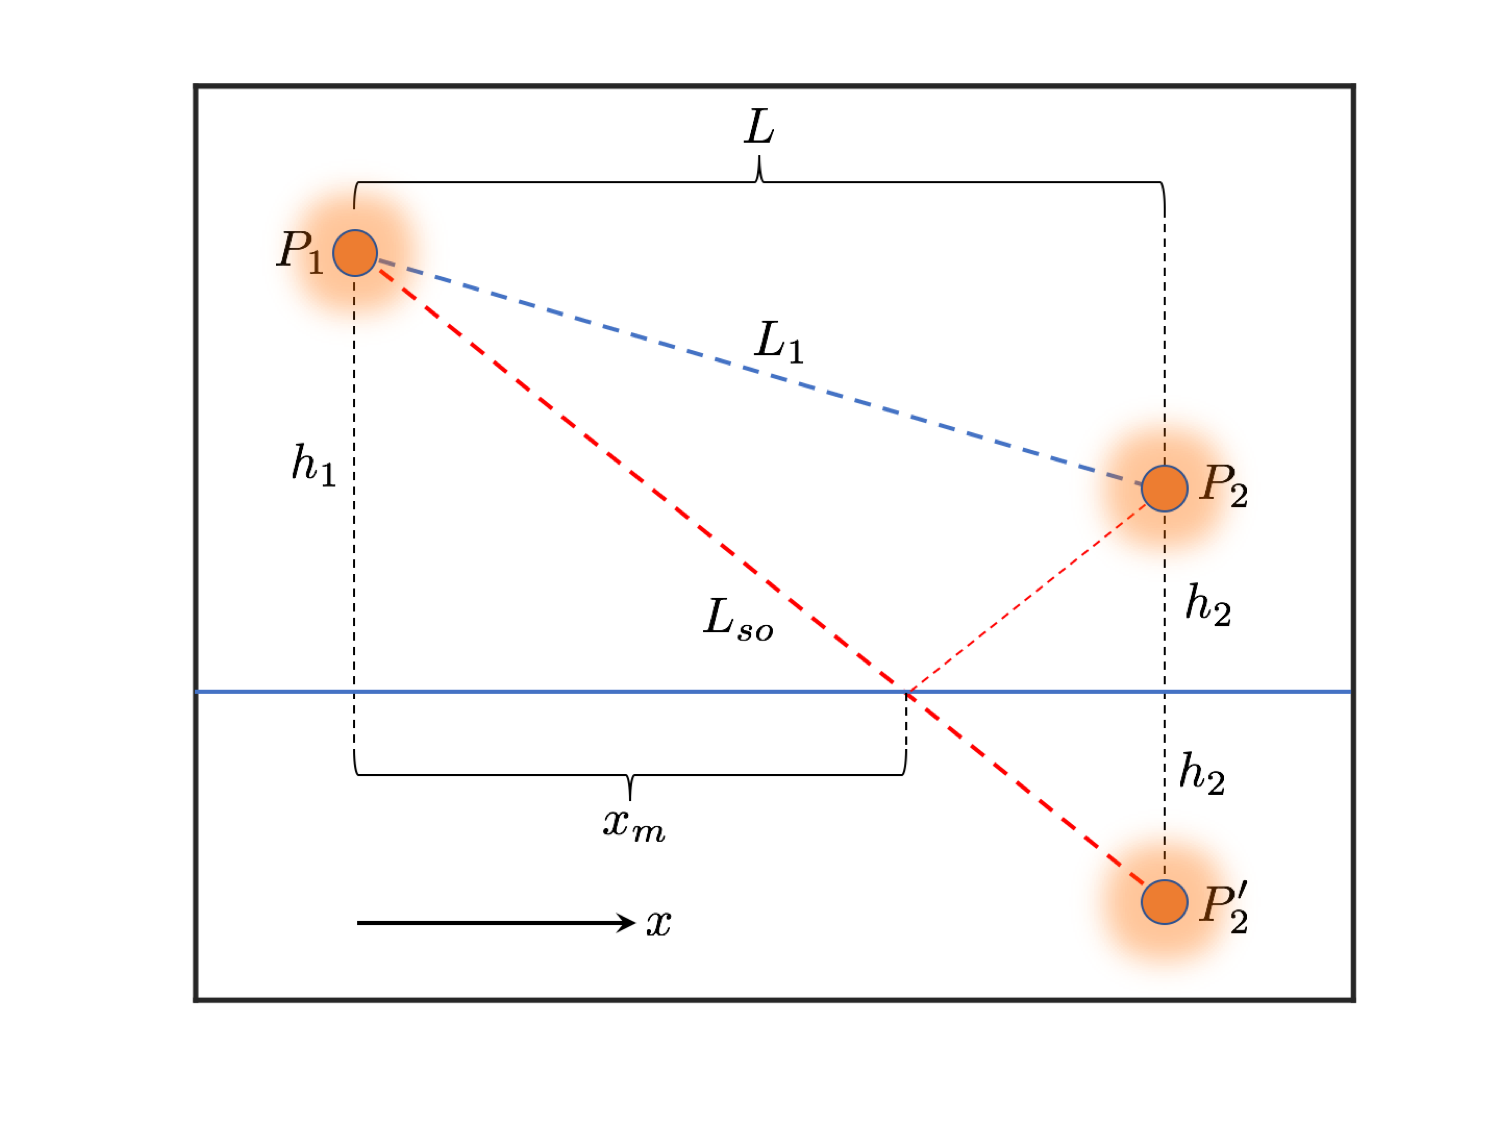
\includegraphics[width=5in]{../media/analysis/multipath_2_ray.png}
  \end{center}
  \renewcommand{\baselinestretch}{1} \small\normalsize
  \begin{quote}
    \caption[2 Ray Multipath Geometry]{ 2 Ray Multipath Geometry\label{mp_fig:1}}
  \end{quote}
\end{figure}
\renewcommand{\baselinestretch}{2} \small\normalsize

To capture the effects of propagating over a spherical earth, the altitude $h_2$ can be modified with a correction factor \cite{blake_radar} dependent on the effective radius of the earth, $r_e = (4/3) 6,371,000$ m.
\begin{equation}
h_2' = h_2 - \frac{L^2}{2r_e}
\label{mp_eq:0}
\end{equation}

The path lengths are given by geometry and simplified through a binomial expansion.
\begin{equation}
\begin{aligned}
L_1 & = \sqrt{L^2 + (h_1-h_2)^2}  \approx L + \frac{(h_1 - h_2)^2}{2L}\\
L_{so} & = \sqrt{L^2 + (h_1+h_2)^2}  \approx L + \frac{(h_1 + h_2)^2}{2L}\\
\end{aligned}
\label{mp_eq:1}
\end{equation}
\renewcommand{\baselinestretch}{2} \small\normalsize

From Huygen's principle, the propagation factor for the 2-ray model is the sum of plane waves traveling along the paths $L_1$ and $L_{so}$. Here $\Gamma_1$ is the reflection coefficient from the sea surface, $\Gamma_1 = \Gamma(x_m)$.
\begin{equation}
\boxed{F_p = e^{ikL_1} + \Gamma_1e^{ikL_{so}}}
\label{mp_eq:1b}
\end{equation}

We can now look at the phase difference between the two primary paths, $\Delta\varphi = k\left[ L_1 - L_{so}\right]$.
\begin{equation}
\boxed{\Delta\varphi = -\frac{4\pi h_1h_2}{\lambda L}}
\label{mp_eq:7}
\end{equation}
\renewcommand{\baselinestretch}{2} \small\normalsize

\noindent The derivative of the phase difference with respect to range is then
\begin{equation}
\frac{d\Delta\varphi}{dL}=-\frac{4\pi h_1h_2}{\lambda L^2}
\label{mp_eq:8}
\end{equation}

\noindent This can be converted from rad/m to rad/sample by multiplying by the spatial sampling distance in range, $\Delta L$. We can insist that this phase shift per sample be smaller than some pre-determined value to provide adequate sampling. It is often convenient to specify a limit in terms of wavelengths and we can enforce the condition that there must be at least $n$ samples per wavelength by letting

\begin{equation}
\frac{4\pi h_1h_2\Delta L}{\lambda L^2} \leq \frac{2\pi \lambda}{n}
\label{mp_eq:10}
\end{equation}

This yields a constraint for the maximum allowable spatial sampling step to ensure $n$ samples per wavelength.
\begin{equation}
\boxed{\Delta L \leq \frac{\lambda^2 L^2}{2nh_1h_2}}
\label{mp_eq:11}
\end{equation}

\section{Multiple Ray Model}
To include multiple rays, we must consider the region over which the electromagnetic wave reflects from the surface, $\tilde{x}$, as shown in Figure \ref{mp_fig:2}. This figure extends Figure \ref{mp_fig:1}, and  $L_2$ and $L_3$ are the path lengths for the various reflected rays and $s(x)$ is the altitude of the sea surface at $x$. 

\begin{figure}[H]
  \begin{center}
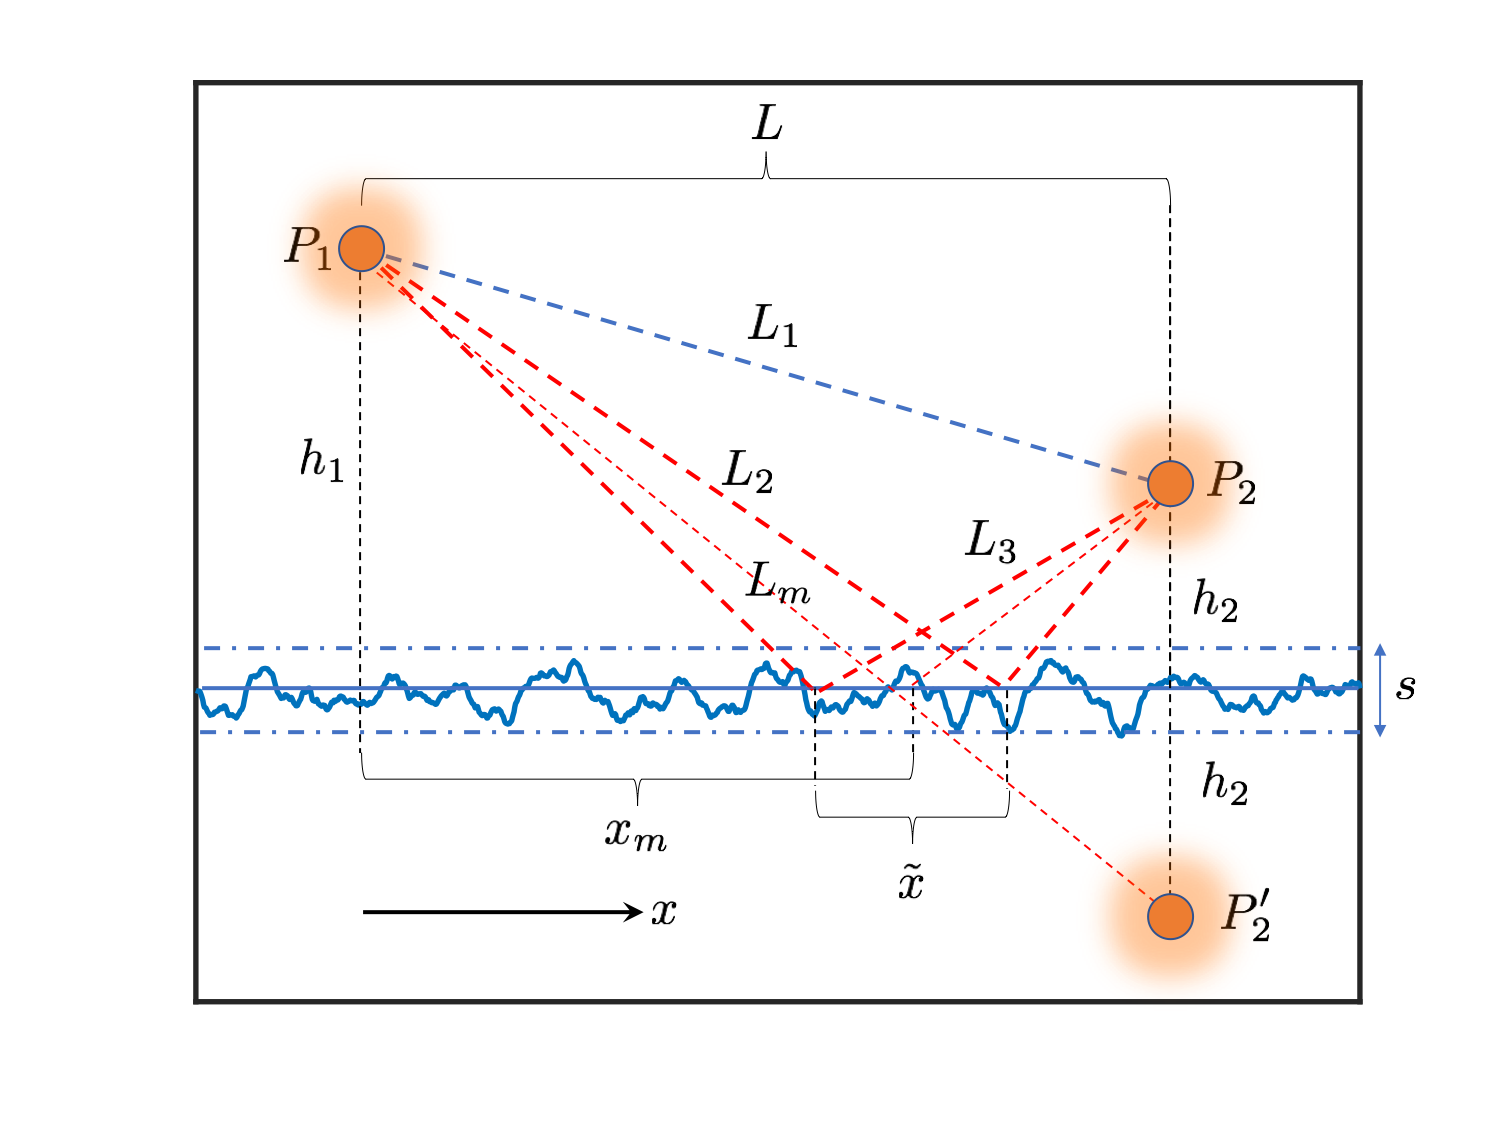
\includegraphics[width=5in]{../media/analysis/multipath_layout.png}
  \end{center}
  \renewcommand{\baselinestretch}{1} \small\normalsize
  \begin{quote}
    \caption[Multipath Geometry for Multiple Ray Analysis]{Multipath Geometry for Multiple Ray Analysis\label{mp_fig:2}}
  \end{quote}
\end{figure}
\renewcommand{\baselinestretch}{2} \small\normalsize

The path lengths  $L_2$ and $L_3$ for the reflected ray can be defined through similar triangles around $x$ and can again be simplified through a binomial expansion. At high altitudes or small sea states, $2h_1s(x) >> s^2(x)$ and we can neglect the $s^2(x)$ term.
\begin{equation}
\begin{aligned}
L_2 &= \sqrt{x^2 + \left( h_1 - s(x)\right)^2}  \approx x + \frac{h_1-s(x))^2}{2x}\\
L_3 & = \sqrt{\left(L - x\right)^2 + \left( h_2 - s(x)\right)^2}  \approx L-x + \frac{h_2 - s(x))^2}{2\left(L-x\right)}\\
\end{aligned}
\label{mp_eq:12}
\end{equation}
\renewcommand{\baselinestretch}{2} \small\normalsize

To solve the propagation problem in the geometry of Figure \ref{mp_fig:2a}, we will find the Green's function for the path from the surface to the receiver and then leverage reciprocity to find the Green's function for the forward path.

\subsection{Green's Function Derivation}
Following Huygen's principle, we can use every point on the sea surface as a source for the reflected wave with the geometry shown in Figure \ref{mp_fig:2a}. Here $\theta$ is defined as the angle between the propagation direction ($\hat{\eta}$) and the direction towards the receiver ($\hat{r}$), and $s$ is the portion of the sea surface that acts as a source. We are assuming here that the region around the reflection point is linear. We are using $\eta$ and $\xi$ as coordinates to prevent confusion with $x$ and $z$ when we introduce them later.

\begin{figure}[H]
  \begin{center}
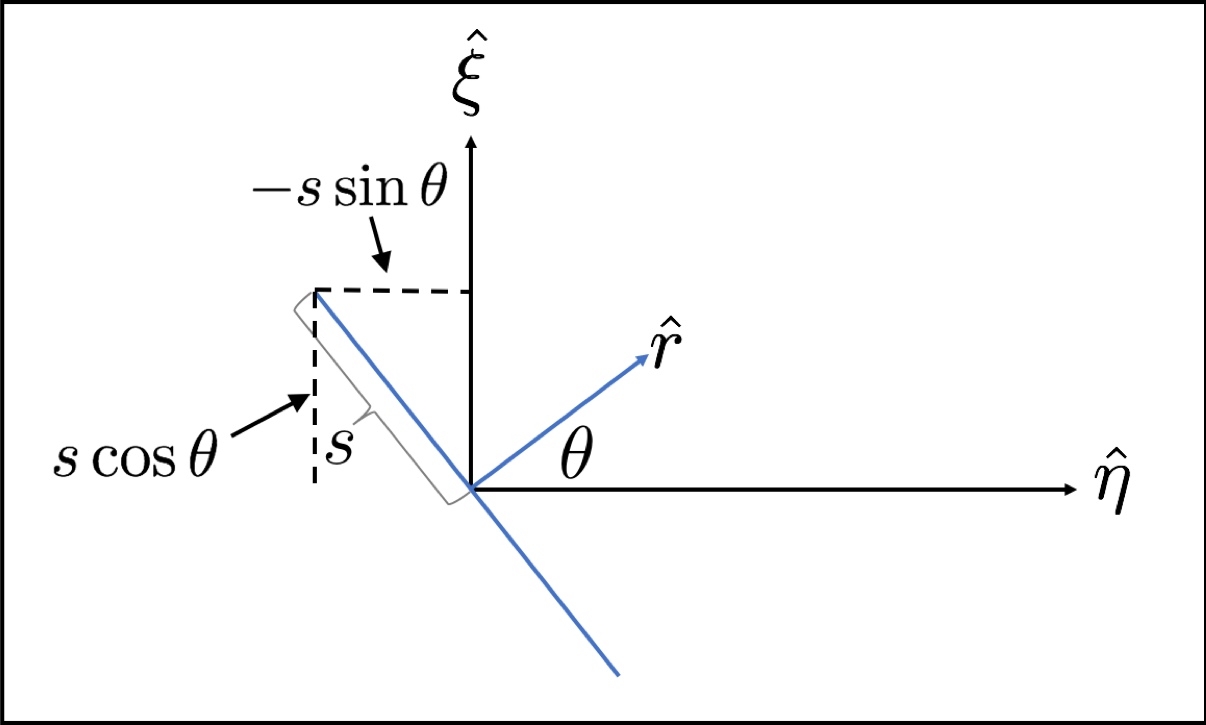
\includegraphics[width=3in]{../media/analysis/gf_geometry.png}
  \end{center}
  \renewcommand{\baselinestretch}{1} \small\normalsize
  \begin{quote}
    \caption[Green's Function Geometry ]{Green's Function Geometry\label{mp_fig:2a}}
  \end{quote}
\end{figure}
\renewcommand{\baselinestretch}{2} \small\normalsize

The projection of $s$ along $\hat{\eta}$ and $\hat{\xi}$ is $-s\sin\theta$ and $s\cos\theta$ respectively. The Green's function can then be computed through the paraxial wave equation with the source constrained along $s$.

\begin{equation}
2jk_o \frac{\partial G}{\partial \eta} - \frac{\partial^2 G}{\partial \xi^2} = -\delta(\eta + s \sin\theta)\delta(\xi - s \cos\theta)
\label{mp_eq:11a}
\end{equation}

We can apply a coordinate transformation of $\eta' = \eta + s\sin\theta$ and $\xi' = \xi - s\cos\theta$
\begin{equation}
2jk_o \frac{\partial G}{\partial \eta'} - \frac{\partial^2 G}{\partial \xi'^2} = -\delta(\eta')\delta(\xi')
\label{mp_eq:11aa}
\end{equation}

Through reciprocity, the Green's function derived in Equation \ref{mp_eq:11fa} can represent the propagation either to the surface or from the surface. With the appropriate selection of $\eta$, $\xi$, and $\theta$, Green's functions for both the forward and reflected paths can be derived. The full Green's function will then be the product of the Green's functions for the individual paths.

\subsection{Solution of the Wave Equation}
To solve the wave equation, we can make the assumption that the sea surface $s$ is small compared to the altitudes, $h_1$ and $h_2$. This means that $s$ will affect the height of the reflection point but have a negligible impact on the surface normal. Therefore we can integrate over $x$ and apply a Dirichlet boundary condition on $G: G|_s = 0$. Since our Greens' function also satisfies the Sommerfeld radiation condition ($\lim_{r\rightarrow\infty} r\left(\frac{\partial G}{\partial r} -ik_oG\right)= 0$) and the outward surface normal is $-\hat{\xi}$

\begin{equation}
U(\bar{r}) = -\int d\eta U(0) \hat{n} \cdot \nabla G = \int d\eta U(0) \frac{\partial G}{\partial \xi}
\label{mp_eq:12a}
\end{equation}

We can take the derivative with respect to $\xi$ of $G$
\begin{equation}
\begin{aligned}
\frac{\partial G}{\partial \xi} &= \frac{j}{2k_o}\sqrt{\frac{k_o}{j2\pi(\eta+s\sin\theta)}}\frac{jk_o2(\xi-s\cos\theta)}{2(\eta+s\sin\theta)}\exp\left[\frac{jk_o(\xi-s\cos\theta)^2}{2(\eta+s\sin\theta)}\right]\\
&= -\sqrt{\frac{k_o}{j2\pi(\eta+s\sin\theta)}}\frac{(\xi-s\cos\theta)}{2(\eta+s\sin\theta)}\exp\left[\frac{jk_o(\xi-s\cos\theta)^2}{2(\eta+s\sin\theta)}\right]\\
\end{aligned}
\label{mp_eq:12b}
\end{equation}

For the first path, we can let the source at $0$ be a plane wave so that $U(0) = e^{jk_o\eta}$
\begin{equation}
U_1(\bar{r}) =  -\int_{0} ^{x_m} d\eta e^{jk_o\eta} \sqrt{\frac{k_o}{j2\pi(\eta+s\sin\theta)}}\frac{(\xi-s\cos\theta)}{2(\eta+s\sin\theta)}\exp\left[\frac{jk_o(\xi-s\cos\theta)^2}{2(\eta+s\sin\theta)}\right]
\label{mp_eq:12c}
\end{equation}

Now we can simplify this expression. In the paraxial approximation, $\cos\theta \approx 1$ and $\sin\theta \approx 0$ and for the first path, $\xi \rightarrow h_1$ and $\eta\rightarrow x$.
\begin{equation}
U_1(\bar{r}) =  -\int_{0} ^{x_m} dx e^{jk_ox} \sqrt{\frac{k_o}{j2\pi x}}\frac{(h_1-s)}{2x}\exp\left[\frac{jk_o(h_1-s)^2}{2x}\right]
\label{mp_eq:12d}
\end{equation}

To add the second path, we will use $U_1$ as the source and add the reflection coefficient from the surface, $\Gamma$.
\begin{equation}
U(\bar{r}) =  -\int_{x_m}^L d\eta \Gamma U_1e^{jk_o\eta} \sqrt{\frac{k_o}{j2\pi(\eta+s\sin\theta)}}\frac{(\xi-s\cos\theta)}{2(\eta+s\sin\theta)}\exp\left[\frac{jk_o(\xi-s\cos\theta)^2}{2(\eta+s\sin\theta)}\right]
\label{mp_eq:12e}
\end{equation}

As in Equation \ref{mp_eq:12d}, for the second path, $\xi \rightarrow h_2$ and $\eta\rightarrow L-x$.
\begin{equation}
U(\bar{r}) =  -\int_{x_m}^L dx \Gamma U_1 e^{jk_o(L-x)}\sqrt{\frac{k_o}{j2\pi(L-x)}}\frac{(h_2-s)}{2(L-x)}\exp\left[\frac{jk_o(h_2-s)^2}{2(L-x)}\right]
\label{mp_eq:12e}
\end{equation}

Expanding and simplifying yields
\begin{equation}
\begin{gathered}
U(\bar{r}) =  -\int_{x_m}^L dx \Gamma\left(-\int_{0} ^{x_m} dx e^{jk_ox} \sqrt{\frac{k_o}{j2\pi x}}\frac{(h_1-s)}{2x}\exp\left[\frac{jk_o(h_1-s)^2}{2x}\right]\right)  \\e^{jk_o(L-x)}\sqrt{\frac{k_o}{j2\pi(L-x)}}\frac{(h_2-s)}{2(L-x)}\exp\left[\frac{jk_o(h_2-s)^2}{2(L-x)}\right]\\
U(\bar{r}) =  \int_{0}^L dx \Gamma e^{jk_oL} \sqrt{\frac{k_o}{j2\pi x}}\frac{(h_1-s)}{2x}\exp\left[\frac{jk_o(h_1-s)^2}{2x}\right]  \\\sqrt{\frac{k_o}{j2\pi(L-x)}}\frac{(h_2-s)}{2(L-x)}\exp\left[\frac{jk_o(h_2-s)^2}{2(L-x)}\right]\\
\end{gathered}
\label{mp_eq:12f}
\end{equation}

We can use the definitions for $L_2$ and $L_3$ from Equation \ref{mp_eq:12} to reduce this further and provide the final integral for $U(\bar{r})$.
\begin{equation}
\boxed{U(\bar{r}) =  \int_{0}^L dx \Gamma \sqrt{\frac{k_o}{j2\pi x}}\sqrt{\frac{k_o}{j2\pi(L-x)}}\frac{(h_1-s)}{2x}\frac{(h_2-s)}{2(L-x)}e^{jk(L_2+L_3)}}
\label{mp_eq:12g}
\end{equation}

\subsection{Approximations}
The path length for a given reflected ray, $L_r$ is then given by
\begin{equation}
\begin{aligned}
L_r &= L_2 + L_3 \\
& = x + \frac{h_1^2-2h_1s(x)}{2x} +  L-x + \frac{h_2^2 - 2h_2s(x)}{2\left(L-x\right)} \\
& = L + \frac{1}{2}\left[\frac{h_1^2}{x} + \frac{h_2^2}{L-x} \right] - s(x)\left[ \frac{h_1}{x} + \frac{h_2}{L-x}\right] \\
&= L + L_0 - L_s
\end{aligned}
\label{mp_eq:13}
\end{equation}
\renewcommand{\baselinestretch}{2} \small\normalsize

Here $L_0$ represents the deterministic component due to reflection from the surface and $L_s$ represents the random component due to reflection from the surface. The reflection point from the 2-ray model, $x_m$, should be a saddle point and provide the dominant contribution. We can therefore perform a Taylor expansion of $L_0$ about $x_m$.

\begin{equation}
L_0 \approx L_0(x_m) + \frac{1}{2}\frac{d^2L_0}{dx^2}\bigg|_{x_m}(x-x_m)^2
\label{mp_eq:14}
\end{equation}

\begin{equation}
\frac{dL_0}{dx} = \frac{1}{2}\left[\frac{-h_1^2}{x^2} + \frac{h_2^2}{(L-x)^2} \right]
\label{mp_eq:15}
\end{equation}

\begin{equation}
\frac{d^2L_0}{dx^2} = \frac{h_1^2}{x^3} + \frac{h_2^2}{(L-x)^3} 
\label{mp_eq:16}
\end{equation}

Since $\frac{dL_0}{dx}\big|_{x_m} = 0$, we can solve for $x_m$
\begin{equation}
\begin{gathered}
\frac{-h_1^2}{x_m^2} + \frac{h_2^2}{(L-x_m)^2} = 0\\
\frac{-h_1}{x_m} + \frac{h_2}{L-x_m} = 0\\
\frac{h_1}{x_m} = \frac{h_2}{L-x_m}\\
h_1(L-x_m) = h_2x_m\\
x_m = \frac{h_1L}{h_1+h_2}
\end{gathered}
\label{mp_eq:17}
\end{equation}

This gives the following for the lowest Taylor series terms:

\begin{equation}
\begin{aligned}
L_0(x_m) &= \frac{(h_1+h_2)^2}{2L} \\
\frac{d^2L_0}{dx^2}\big|_{x_m}  &= \frac{(h_1+h_2)^4}{h_1h_2L^3} \\
L_s(x_m) &= \frac{2s(x)(h_1 + h_2)}{L}\\
\end{aligned}
\label{mp_eq:17a}
\end{equation}

The expansion of $L_0$ is then
\begin{equation}
L_0 \approx \frac{(h_1+h_2)^2}{2L} + \frac{(h_1+h_2)^4}{2h_1h_2L^3}(x-x_m)^2
\label{mp_eq:18}
\end{equation}

The propagation factor will now include all the reflections from the surface

\begin{equation}
\begin{aligned}
F_p &= e^{ikL_1} + \int_0^Ldx\Gamma  e^{ik(L_2+L_3)}\\
&= e^{ikL_1} + \int_0^Ldx\Gamma  e^{ik(L+L_0-L_s)}\\
&= e^{ikL_1} +  \Gamma_1e^{ik(L+\frac{(h_1+h_2)^2}{2L})}\int_0^Ldx\frac{\Gamma}{\Gamma_1} e^{ik(\frac{L_0''}{2}(x-x_m)^2-L_s)}\\
&= e^{ikL_1} + \Gamma_1e^{ikL_{so}}\int_0^Ldx\frac{\Gamma}{\Gamma_1} \exp\left[\frac{ikL_0''}{2}(x-x_m)^2 - \frac{i2ks(x)(h_1+h_2)}{L}\right]\\
\end{aligned}
\label{mp_eq:20}
\end{equation}

We have a similar expression to Equation \ref{mp_eq:1b} with the propagation factor from the shortest orbit reflection scaled by contributions from all the other reflected rays. letting $x-x_m \rightarrow \tilde{x}$, we can express the propagation factor as

\begin{equation}
\boxed{F_p = e^{ikL_1} + \Gamma_1 e^{ikL_{so}}\int_{-x_m}^{L-x_m}d\tilde{x} \frac{\Gamma(\tilde{x})}{\Gamma_1}\exp\left[\frac{ikL_0''}{2}\tilde{x}^2 - \frac{i2ks(\tilde{x})(h_1+h_2)}{L}\right]}
\label{mp_eq:21}
\end{equation}

\section{Asymptotic Approach for Deterministic Component}
For the deterministic component, we wish to solve the integral given by
\begin{equation}
I = \int_{-x_m}^{L-x_m}d\tilde{x} \frac{\Gamma(\tilde{x})}{\Gamma_1}\exp\left[\frac{ikL_0''}{2}\tilde{x}^2\right]
\label{mp_eq:22}
\end{equation}

The phase of the integrand oscillates rapidly as shown by the real part of the integrand in Figure \ref{mp_fig:3} with a 10m altitude target, Figure \ref{mp_fig:4} with a 20m altitude target and Figure \ref{mp_fig:5} with a 50m altitude target. Each subplot shows the impact of increasing the ground distance, $L$, with the lower right subplot showing the horizon limit.

\begin{figure}[H]
  \begin{center}
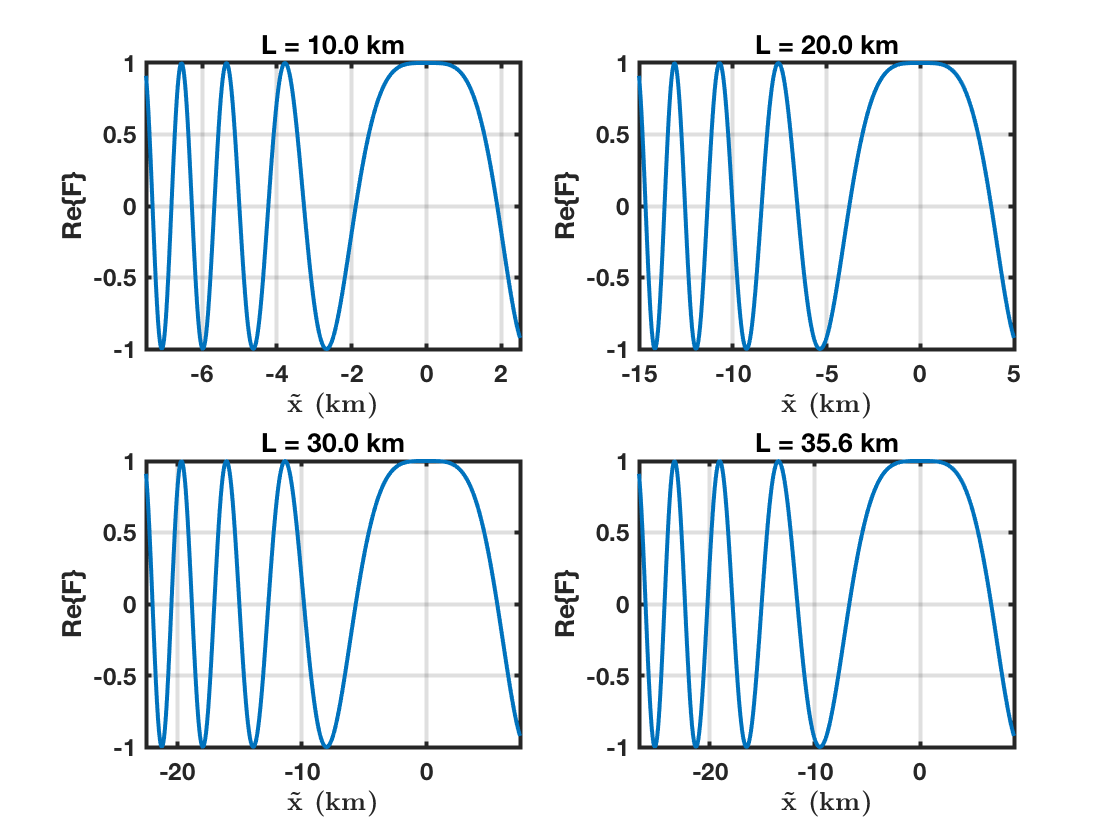
\includegraphics[width=4in]{../media/analysis/phaseVariation_30_10}
  \end{center}
  \renewcommand{\baselinestretch}{1} \small\normalsize
  \begin{quote}
    \caption[Real Part of Integrand for $h_1$ = 30m, $h_2$ = 10m]{ Real Part of Integrand for $h_1$ = 30m, $h_2$ = 10m\label{mp_fig:3}}
  \end{quote}
\end{figure}
\renewcommand{\baselinestretch}{2} \small\normalsize

\begin{figure}[H]
  \begin{center}
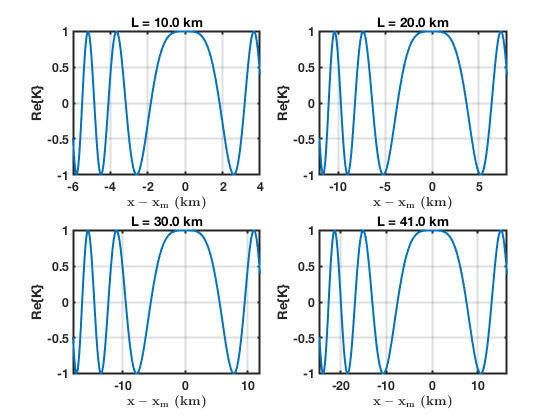
\includegraphics[width=4in]{../media/analysis/phaseVariation_30_20}
  \end{center}
  \renewcommand{\baselinestretch}{1} \small\normalsize
  \begin{quote}
  \caption[Real Part of Integrand for $h_1$ = 30m, $h_2$ = 20m]{ Real Part of Integrand for $h_1$ = 30m, $h_2$ = 20m\label{mp_fig:4}}
  \end{quote}
\end{figure}
\renewcommand{\baselinestretch}{2} \small\normalsize

\begin{figure}[H]
  \begin{center}
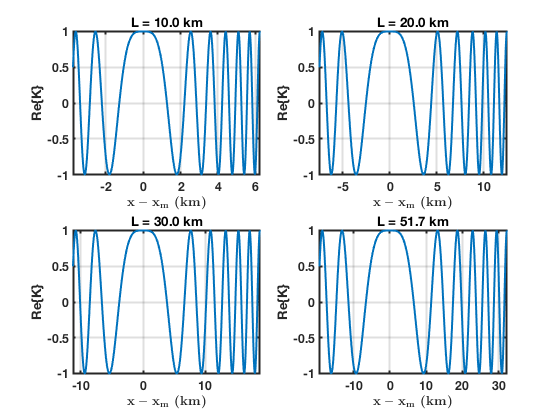
\includegraphics[width=4in]{../media/analysis/phaseVariation_30_50}
  \end{center}
  \renewcommand{\baselinestretch}{1} \small\normalsize
  \begin{quote}
  \caption[Real Part of Integrand for $h_1$ = 30m, $h_2$ = 50m]{ Real Part of Integrand for $h_1$ = 30m, $h_2$ = 10m\label{mp_fig:5}}
  \end{quote}
\end{figure}
\renewcommand{\baselinestretch}{2} \small\normalsize

Even with low altitudes, the phase oscillations will be rapid as $\tilde{x}$ goes past the limits of integration and will cancel out, so we can use the principle of stationary phase and let the limits of integration go to $\pm\infty$. Since the integrand is an even function, we can then take the limit from $0$ to $+\infty$ and multiply by 2.

\begin{equation}
I = \int_{-\infty}^{\infty}d\tilde{x} \frac{\Gamma(\tilde{x})}{\Gamma_1}\exp\left[\frac{ikL_0''}{2}\tilde{x}^2\right] = 2\int_{0}^{\infty}d\tilde{x} \frac{\Gamma(\tilde{x})}{\Gamma_1}\exp\left[\frac{ikL_0''}{2}\tilde{x}^2\right] 
\label{mp_eq:23}
\end{equation}

To solve this equation, we can work in the complex plane as shown in Figure \ref{mp_fig:6}. The contour along the real axis, $\mathcal{C}_1$, is deformed to ensure we do not cross through the singular point at $\tilde{x} = L-x_m$ as given in Equation \ref{mp_eq:13} for the initial expression of $L_0$. From Jordan's Lemma, the contour along the arc $\mathcal{C}_2$ will be $0$. Since there are no singular points enclosed by the contour, the sum of the integrals along the contours is $0$ so that

\begin{equation}
I = -2\int_{\mathcal{C}_3}d\tilde{x} \frac{\Gamma(\tilde{x})}{\Gamma_1}\exp\left[\frac{ikL_0''}{2}\tilde{x}^2\right]  
\label{mp_eq:24}
\end{equation}

\begin{figure}[H]
  \begin{center}
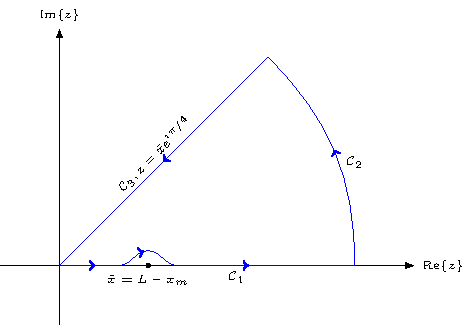
\includegraphics[width=5in]{../media/path_contour-figure0.pdf}
  \end{center}
  \renewcommand{\baselinestretch}{1} \small\normalsize
  \begin{quote}
    \caption[Path Contour]{ Path Contour\label{mp_fig:6}}
  \end{quote}
\end{figure}
\renewcommand{\baselinestretch}{2} \small\normalsize

To ensure we take the path of steepest descent, we can transform $\tilde{x}$ to the complex variable $z$ by applying a phase shift of $\pi/4$. Now we can approximate the integral as

\begin{equation}
\begin{gathered}
I = -2\int_{\mathcal{C}_3}d\tilde{z}e^{i\pi/4} \frac{\Gamma(x_m)}{\Gamma_1}\exp\left[\frac{-kL_0''}{2}\tilde{z}^2\right]  \\
= 2e^{i\pi/4}\int_{0}^{\infty}d\tilde{z}\frac{\Gamma_1}{\Gamma_1}\exp\left[\frac{-kL_0''}{2}\tilde{z}^2\right]  \\
= 2e^{i\pi/4}\sqrt{\frac{2\pi}{kL_o''}}
\end{gathered}
\label{mp_eq:25}
\end{equation}

This yields an asymptotic approximation for the deterministic component of equation \ref{mp_eq:21}.
\begin{equation}
\boxed{F_p = e^{ikL_1} +2\Gamma_1 e^{i\left(kL_{so} + \pi/4\right)}\sqrt{\frac{2\pi}{kL_o''}}}
\label{mp_eq:26}
\end{equation}

\renewcommand{\thechapter}{6}
\chapter{Cylindrical Wave Propagation Model}
\label{cylindrical_propagation}
This section derives the solution for the multiple ray model using cylindrical waves and leverages the results from Chapter \ref{analytical_propagation} for the paraxial wave case.

\section{Solution through Green's Functions}
The Green's function for the cylindrical wave was derived in Section \ref{gf_sec:2d} as
\begin{equation}
G\left(\boldsymbol{\rho},\boldsymbol{\rho}'\right) = -\frac{j}{4}H_0^{(2)}\left(k_o|\boldsymbol{\rho} - \boldsymbol{\rho}' | \right)
\label{cyl_eq:1}
\end{equation}
\renewcommand{\baselinestretch}{2} \small\normalsize

\noindent The source is located at $\boldsymbol{\rho}'$ and the observation point is located at $\boldsymbol{\rho}$. 

\subsection{Direct Path}
Assuming a point source located at $\boldsymbol{\rho}' = (\rho,\theta) = (0,0)$, we can compute the direct path as the volume integral of the product of the Green's function and the source. The delta function in cylindrical coordinates needs to be scaled by the differential volume element to ensure the delta function is properly normalized so its volume integral is equal to $1$.  

\begin{equation}
\begin{aligned}
U_1(P_2) & = \int_{-\infty}^{\infty}\int_0^{2\pi} d\rho' \rho' d\theta' G\frac{\delta(\rho')\delta(\theta')}{\rho'}\\
&-= \int_{-\infty}^{\infty}\int_0^{2\pi} d\rho' \rho' d\theta' \frac{j}{4}H_0^{(2)}\left(k_o|\boldsymbol{\rho} - \boldsymbol{\rho}' | \right)\frac{\delta(\rho')\delta(\theta')}{\rho'}\\
&=-\frac{j}{4}H_0^{(2)}\left(k_o|\boldsymbol{\rho}| \right)
\label{cyl_eq:2}
\end{aligned}
\end{equation}
\renewcommand{\baselinestretch}{2} \small\normalsize

\noindent For the direct path, $|\boldsymbol{\rho}'| = L_1$, so the  solution is
\begin{equation}
U_1(P_2) =-\frac{j}{4}H_0^{(2)}\left(k_oL_1 \right)
\label{cyl_eq:3}
\end{equation}
\renewcommand{\baselinestretch}{2} \small\normalsize

The asymptotic approximation for the Hankel functions were derived in Appendix \ref{appendix_saddle_point_method} for large arguments
\begin{equation}
H_{\nu}^{(2)}(k_oL) \approx \sqrt{\frac{2}{\pi k_o L}}e^{-j\left[k_oL - \nu\frac{\pi}{2} - \frac{\pi}{4}\right]}
\label{cyl_eq:4}
\end{equation}
\renewcommand{\baselinestretch}{2} \small\normalsize

\noindent For any case of interest, $kL_1$ will be large so we can safely approximate Equation \ref{cyl_eq:3} as
\begin{equation}
\begin{aligned}
U_1(P_2) &=-\frac{j}{4}\sqrt{\frac{2}{\pi k_o L_1}}e^{-j(k_oL_1 - \frac{\pi}{4})}\\
&=-\frac{j}{4}\sqrt{\frac{2}{j\pi k_o}}\frac{1}{\sqrt{L_1}}e^{-jk_oL_1 }\\
&=\frac{\alpha}{\sqrt{L_1}}e^{-jk_oL_1 }\\
\label{cyl_eq:5}
\end{aligned}
\end{equation}
\renewcommand{\baselinestretch}{2} \small\normalsize
Here, we are using a normalization factor, $\alpha$ to take out the common scaling terms when computing the propagation factor. The $1/\sqrt{L_1}$ scale factor introduces the cylindrical spreading.

\subsection{Reflected Path}
For the reflected path, we can again use the Rayleigh-Sommerfeld Diffraction Integral with the solution at the sea surface, $U(s)$, given as $-\frac{j}{4}H_0^{(2)}\left(k_oL_2 \right)$
\begin{equation}
\begin{aligned}
U_2(P_2) &= -2\oint_s ds U_2(s)\hat{n}\cdot\nabla G\\
&= -2\int_0^L dx \Gamma U_2(s)\cos(\phi)\frac{\partial G}{\partial \rho}\\
\end{aligned}
\label{cyl_eq:6}
\end{equation}

From Equation \ref{cyl_eq:5}, $U_2(s) = \alpha/\sqrt{L_2} e^{-jkL_2}$ and we can use the fact that $\partial H_0^{(2)}(k_o\rho)/\partial \rho = -k_oH_1^{(2)}(k_o\rho)$ and $\cos(\phi) = h2/L_3$ to solve for $U_2(P_2)$.
\begin{equation}
\begin{aligned}
U_2(P_2) &= -2\int_0^L dx \Gamma\frac{\alpha}{\sqrt{L_2}}e^{-jk_oL_2}(-k_o)\frac{h_2}{L_3}H_1^{(2)}(k_oL_3)\\
&= -\frac{j}{4}\alpha 2k_o\int_0^L dx \Gamma\frac{h_2}{L_3}\frac{1}{\sqrt{L_2}}e^{-jk_oL_2}\sqrt{\frac{2}{\pi k_o L_3}}e^{-j(k_oL_3-3\pi /4)}\\
&=-\frac{j\alpha h_2k_o }{2}\sqrt{\frac{2}{\pi k_o}}\int_0^L dx\Gamma \frac{1}{L_3\sqrt{L_2L_3}}e^{-jk_o(L_2+L_3)}e^{j3\pi/4}\\
&= \frac{\alpha h_2k_o}{2}\sqrt{\frac{2j}{\pi k_o}}\int_0^L dx\Gamma \frac{h_2}{L_3} \frac{1}{L_3\sqrt{L_2L_3}}e^{-jk_o(L_2+L_3)}\\
&= \alpha h_2\sqrt{\frac{j k_o}{2\pi}}\int_0^L dx \Gamma\frac{1}{L_3\sqrt{L_2L_3}}e^{-jk_o(L_2+L_3)}\\
\end{aligned}
\label{cyl_eq:7}
\end{equation}

We can use the contour integral approach again to get the following solution for the deterministic component where $L_2$ and $L_3$ now imply the values at $x_m$.
\begin{equation}
\begin{aligned}
U_2(P_2) &=\frac{\alpha h_2\Gamma_1}{L_3\sqrt{L_2L_3}}\sqrt{\frac{j k_o}{2\pi}}\sqrt{\frac{2\pi}{j k_oL_0''}}e^{-jk_oL_{so}}\\
&=\frac{\alpha h_2\Gamma_1}{L_3\sqrt{L_2L_3}}\sqrt{\frac{L^3}{(h_1+h_2)^4}}
e^{-jk_oL_{so} }\end{aligned}
\label{cyl_eq:8}
\end{equation}

The normalized propagation factor is then
\begin{equation}
\begin{aligned}
\boxed{F_p =e^{-jk_oL_1} + \frac{h_2\Gamma_1\sqrt{L_1}}{L_3\sqrt{L_2L_3}}\sqrt{\frac{L^3}{(h_1+h_2)^4}}e^{-jk_oL_{so} }}
\end{aligned}
\label{cyl_eq:9}
\end{equation}


\renewcommand{\thechapter}{7}
\chapter{Numerical Propagation}
\label{numerical_propagation}
This chapter describes how the numerical propagation was implemented for this work, starting with an overview of the Parabolic Wave Equation (PWE) before discussing the propagation geometries.

\section{Parabolic Wave Equation}

\section{Geometry}
Figure \ref{np_fig:1} shows an example propagation geometry.
\begin{figure}[H]
  \begin{center} 
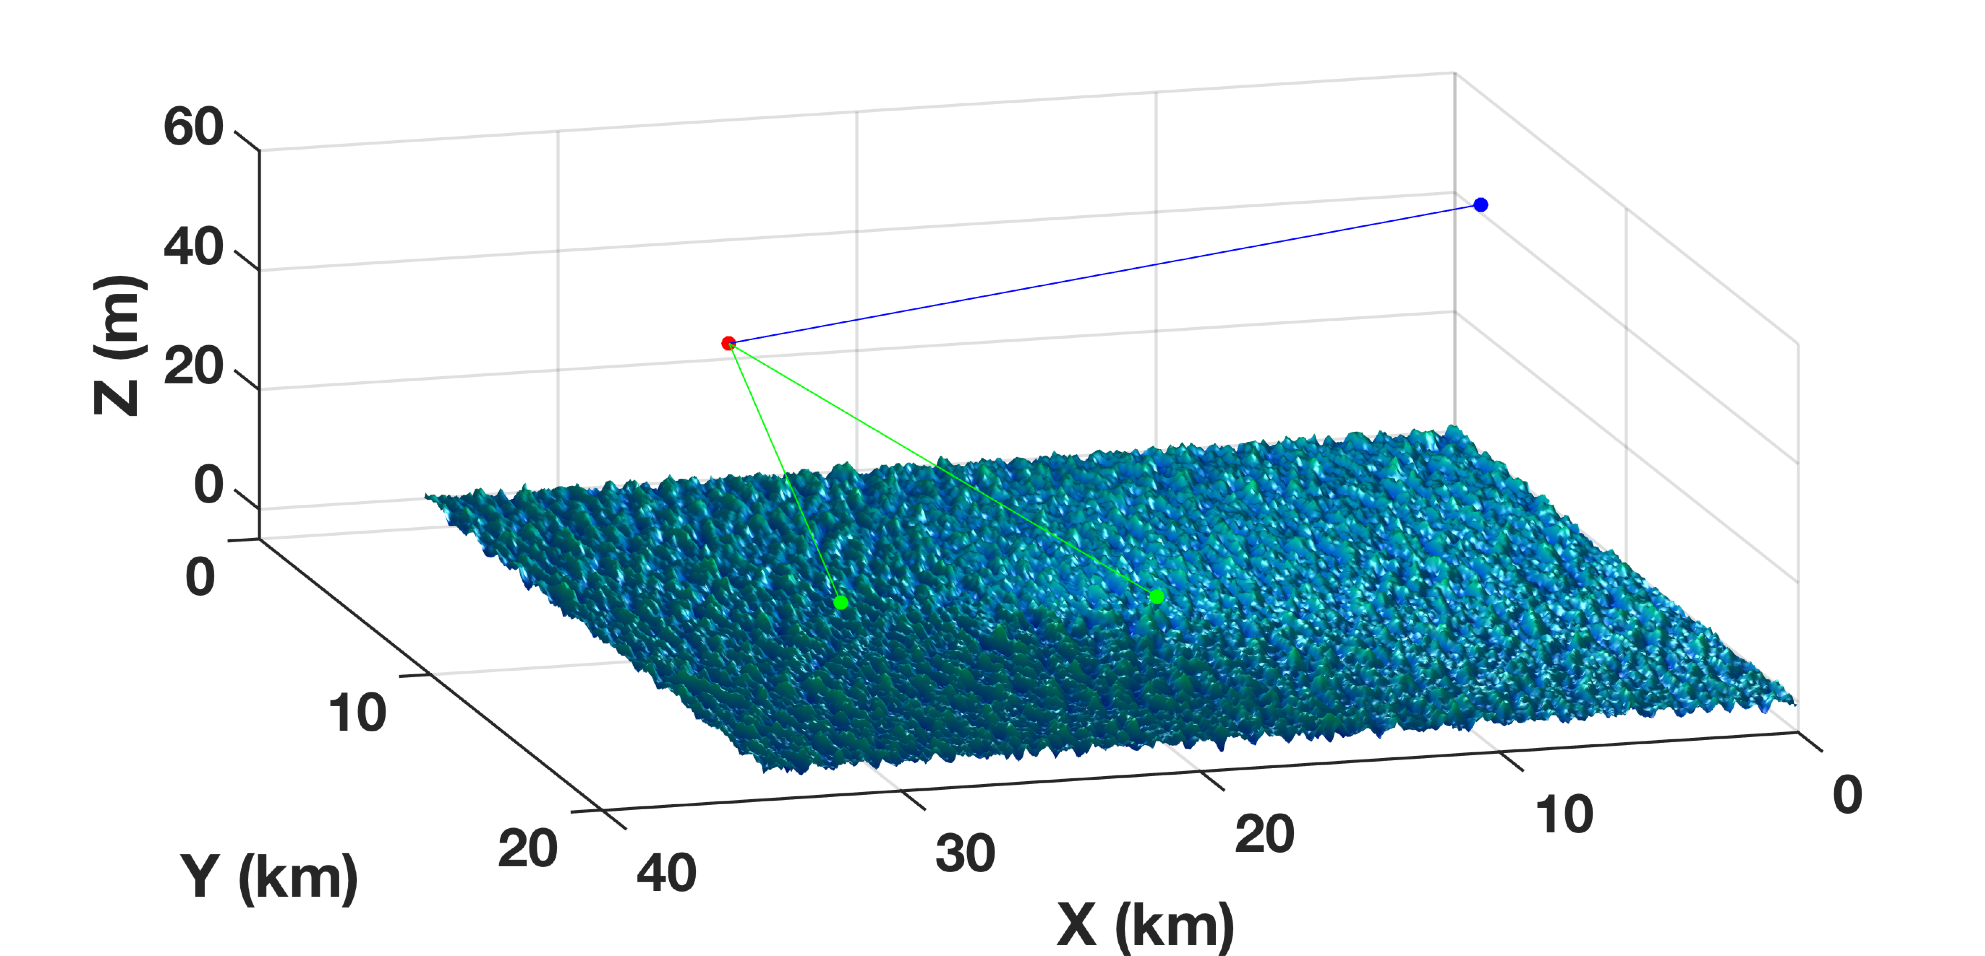
\includegraphics[width=5in]{../media/multistatic/ms_rf_concept2.png}
  \end{center}
  \renewcommand{\baselinestretch}{1} \small\normalsize
  \begin{quote}
    \caption[Example Multi-static Propagation Geometry]{Example Multi-static Propagation Geometry\label{np_fig:1}}
  \end{quote}
\end{figure}
\renewcommand{\baselinestretch}{2} \small\normalsize

Because the receiver and transmitter are not colocated, we cannot leverage reciprocity for the primary path and will need to propagate along both paths. We can however keep the propagation domain to 1-dimension. This is accomplished by generating a sea surface with the wind direction relative to the line of sight between the transmitter and the target for the first path and relative to the line of sight between the receiver and the target for the second path.

\renewcommand{\thechapter}{8}
\renewcommand{\baselinestretch}{2} \small\normalsize
\section{Propagation Statistics}
This chapter describes the propagation factor statistics after numerically propagating over independent random sea surface realizations generated following \cite{frazier_ocean} in a Monte Carlo fashion. First we will discuss the sampling constraints needed to capture the statistics appropriately and then look at the Monte Carlo run setup and provide some example data before finally fitting the PDFs.

\subsection{Sampling Constraints}
The initial set of runs was performed at Ka-Band (35 GHz) and the mean and standard deviation for a 100 run Monte Carlo set are shown in Figure \ref{stat_fig:1}. This data set took over 48 hours to complete running on a laptop and the results were washed out at near range (Figure \ref{stat_fig:1} is clipped at 10 km in near range).

\begin{figure}[H]
  \begin{center}
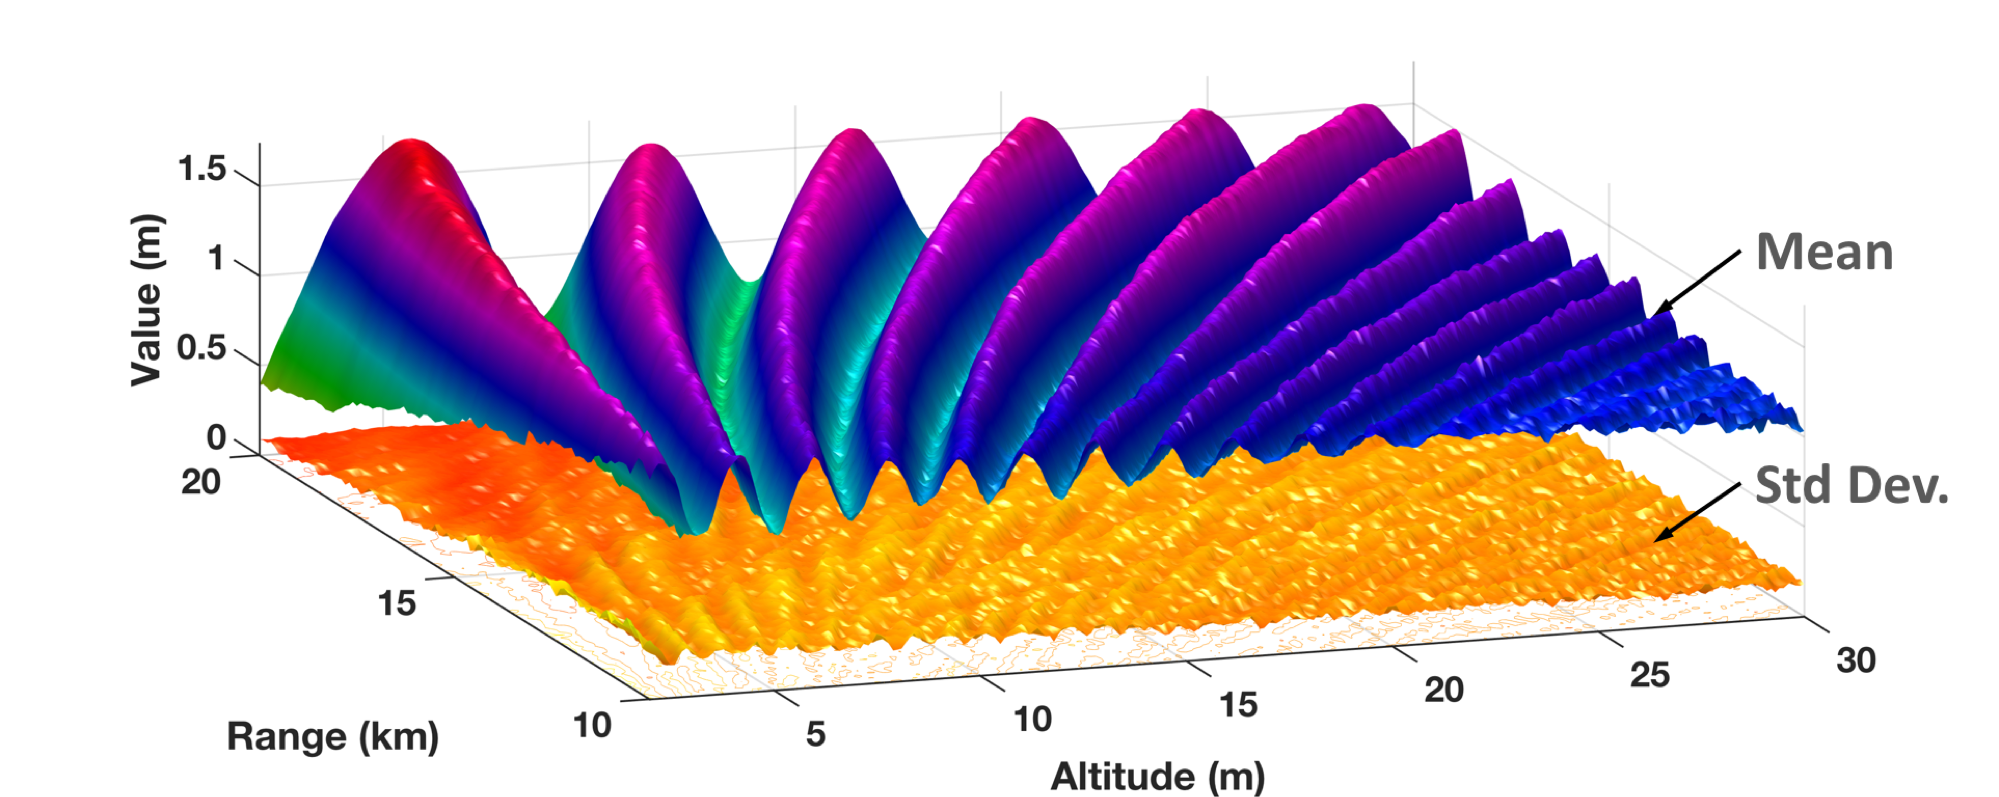
\includegraphics[width=5in]{../media/statistics/ka_band_stats.png}
  \end{center}
  \renewcommand{\baselinestretch}{1} \small\normalsize
  \begin{quote}
    \caption[Ensemble Statistics at Ka-Band with Standard Atmosphere]{Ensemble Statistics at Ka-Band with Standard Atmosphere\label{stat_fig:1}}
  \end{quote}
\end{figure}
\renewcommand{\baselinestretch}{2} \small\normalsize

Figure \ref{stat_fig:2} shows the mean and standard deviation for a 100 run Monte Carlo set at X-band (10 GHz). In this case, the near range results are much cleaner and the data set took less than 6 hours to complete.
\begin{figure}[H]
  \begin{center}
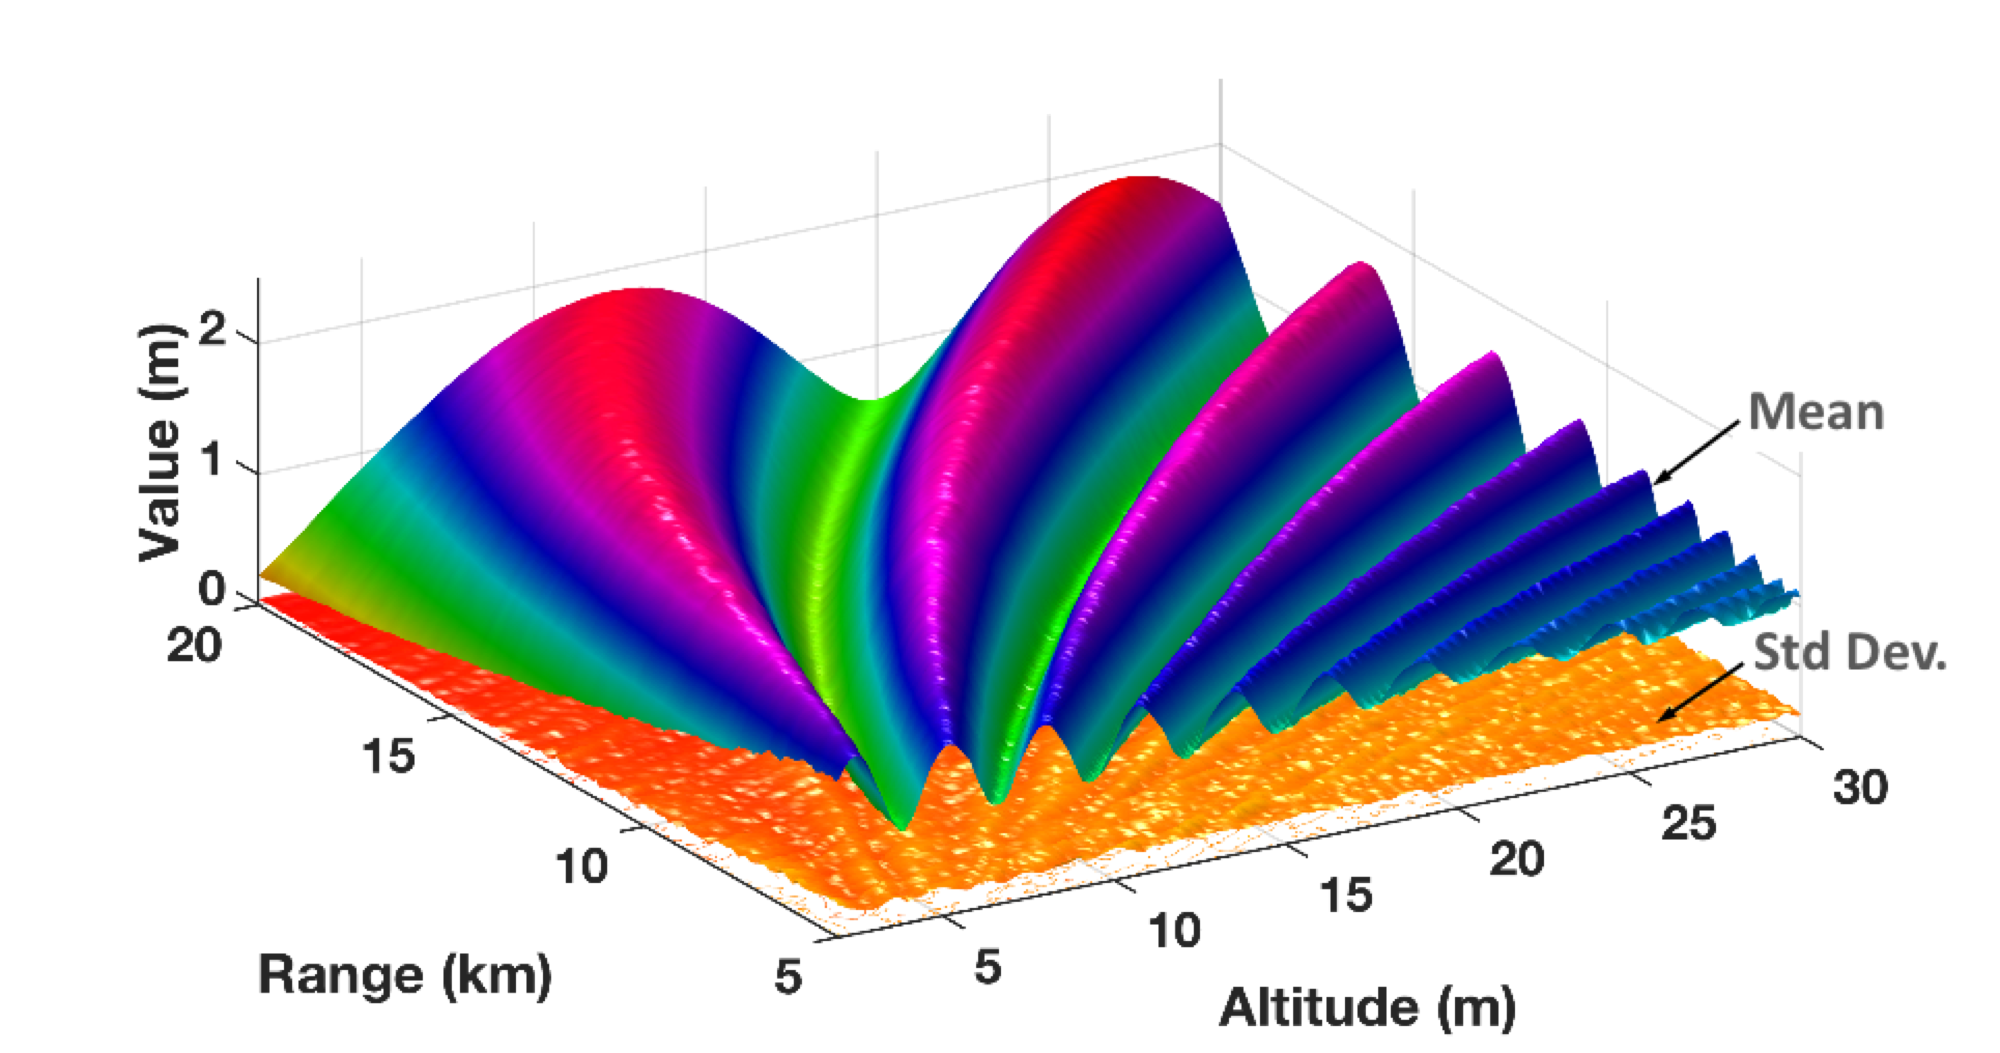
\includegraphics[width=5in]{../media/statistics/x_band_stats.png}
  \end{center}
  \renewcommand{\baselinestretch}{1} \small\normalsize
  \begin{quote}
    \caption[Ensemble Statistics at X-Band with Standard Atmosphere]{Ensemble Statistics at X-Band with Standard Atmosphere\label{stat_fig:2}}
  \end{quote}
\end{figure}
\renewcommand{\baselinestretch}{2} \small\normalsize

These results indicate that spatial sampling constraints from numerical propagation are important for obtaining accurate statistics. This does not mean the numerical propagation method is inaccurate, but that the solution is locally oscillatory so we need finer sampling to correctly capture variations.

To investigate the sampling constraints, we can look at the phase difference between the two primary paths from the propagation factor for the 2 ray model, $F_p = e^{jkL_1} + \Gamma_1e^{jkL_{so}}$. 

\begin{equation}
\begin{gathered}
\Delta\varphi = k\left[ L_1 - L_{so}\right] \\
\Delta\varphi = -\frac{4\pi h_1h_2}{\lambda L}
\label{stat_eq:1}
\end{gathered}
\end{equation}
\renewcommand{\baselinestretch}{2} \small\normalsize

The derivative of the phase difference with respect to range is then

\begin{equation}
\frac{d\Delta\varphi}{dL}=\frac{4\pi h_1h_2}{\lambda L^2}
\label{stat_eq:2}
\end{equation}
\renewcommand{\baselinestretch}{2} \small\normalsize

\noindent This equation can be converted from rad/m to rad/sample by multiplying by the spatial sampling distance in range, $\Delta r$. We can insist that this phase shift per sample be smaller than some pre-determined value to provide adequate sampling. It is often convenient to specify a limit in terms of wavelengths and we can enforce the condition that there must be at least $n$ samples per wavelength of phase difference by letting

\begin{equation}
\frac{4\pi h_1h_2\Delta r}{\lambda L^2} \leq \frac{2\pi \lambda}{n}
\label{stat_eq:3}
\end{equation}

This yields a constraint for the maximum allowable spatial sampling step to ensure $n$ samples per wavelength.
\begin{equation}
\boxed{\Delta r \leq \frac{\lambda^2 L^2}{2nh_1h_2}}
\label{stat_eq:4}
\end{equation}

This equation matches the observation with $n\approx 10$ for the mean values and $n\approx 20$ for the standard deviations. The sampling constraint is shown in Figure \ref{stat_fig:3} for both the 10 and 35 GHz cases, with $n = 20$ and $\Delta r = 0.5$.

\begin{figure}[H]
  \begin{center}
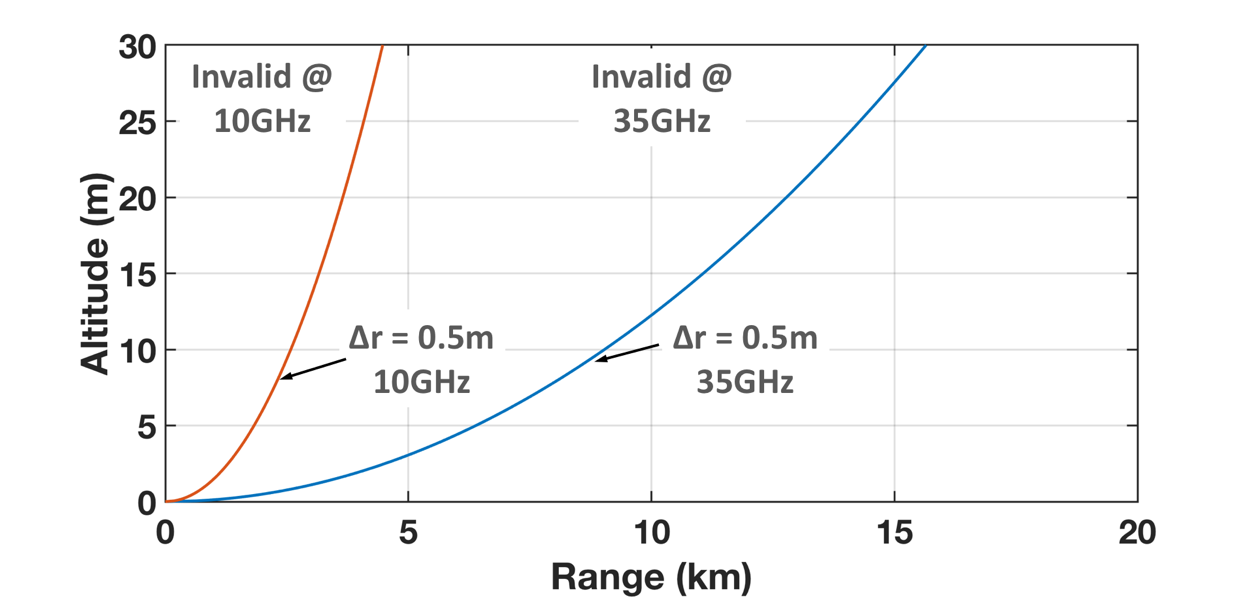
\includegraphics[width=5in]{../media/statistics/sampling_constraint.png}
  \end{center}
  \renewcommand{\baselinestretch}{1} \small\normalsize
  \begin{quote}
    \caption[Sampling Constraints for Statistical Analysis]{Sampling Constraints for Statistical Analysis\label{stat_fig:3}}
  \end{quote}
\end{figure}
\renewcommand{\baselinestretch}{2} \small\normalsize

In order to reduce the sampling constraints and run the Monte Carlo study in a reasonable amount of time, the temporal frequency of interest was changed from 35 GHz to 10 GHz.

\subsection{Monte Carlo Run Methodology}
The data set of propagation factors were generated by creating a random sea surface for a given wind speed and direction, and then numerically propagating using TEMPER. This sequence was repeated for 500 iterations with a different set of random variables for each sea surface.

\subsubsection{Input Parameters}
Table \ref{stat_tab:0} shows the common inputs that were used in all of the Monte Carlo runs.

\begin{table}[H]
  \begin{center}
      \renewcommand{\baselinestretch}{1} \small\normalsize
  \begin{quote}
    \caption[Common Monte Carlo Input Settings]{Common Monte Carlo Input Settings\label{stat_tab:1}}
  \end{quote}
  \begin{tabular} {|c | c |}
    \hline
  \bf{Parameter} & \bf{Value} \\ \hline
  Frequency & 10 GHz \\ \hline
  Antenna Pattern & Sinc \\ \hline
  Antenna Beamwidth & $8^{\circ}$  \\ \hline
  Polarization & Vertical \\ \hline
  Transmitter Height & 30 m \\ \hline
  Maximum Range & 20 km \\ \hline
  Range Step & 0.5 m  \\ \hline
  Maximum Altitude & 30 m \\ \hline
  Earth Model & Spherical \\ \hline
  Inverse Age Parameter & 0.84 (fully developed) \\ \hline
  Initial Seed & 561894\\ \hline
  Number of Runs & 500\\ \hline
\end{tabular}
\end{center}
\end{table}
\renewcommand{\baselinestretch}{2} \small\normalsize

The parameterizations resulted in 26 total data sets to capture the effect of wind speed (from 2 m/s to 15 m/s at $0^{\circ}$ wind direction), wind direction ($90^{\circ}$ to $0^{\circ}$ at 10 m/s wind speed), and refractive index profile (standard atmosphere and a 20 m duct). Table \ref{stat_tab:1} shows the primary run matrix with the various parameterizations. 

\begin{table}[H]
  \begin{center}
      \renewcommand{\baselinestretch}{1} \small\normalsize
  \begin{quote}
    \caption[Monte Carlo Propagation Run Matrix]{Monte Carlo Propagation Run Matrix\label{stat_tab:0}}
  \end{quote}
  \begin{tabular} {|c | c | c| c |}
    \hline
  \bf{Dataset ID} & \bf{Wind Speed} & \bf{Wind Direction} & \bf{Refractivity}  \\ \hline
  1 & 2 m/s & $0^{\circ}$ & Standard Atmosphere \\ \hline
  2 & 3 m/s & $0^{\circ}$ & Standard Atmosphere \\ \hline
  3 & 4 m/s & $0^{\circ}$ & Standard Atmosphere \\ \hline
  4 & 5 m/s & $0^{\circ}$ & Standard Atmosphere \\ \hline
  5 & 8 m/s & $0^{\circ}$ & Standard Atmosphere \\ \hline
  6 & 10 m/s & $0^{\circ}$ & Standard Atmosphere \\ \hline
  7 & 12 m/s & $0^{\circ}$ & Standard Atmosphere \\ \hline
  8 & 15 m/s & $0^{\circ}$ & Standard Atmosphere \\ \hline
  9 & 10 m/s & $18^{\circ}$ & Standard Atmosphere \\ \hline
  10 & 10 m/s & $36^{\circ}$ & Standard Atmosphere \\ \hline
  11 & 10 m/s & $54^{\circ}$ &  Standard Atmosphere\\ \hline
  12 & 10 m/s & $72^{\circ}$ &  Standard Atmosphere \\ \hline
  13 & 10 m/s & $90^{\circ}$ &  Standard Atmosphere \\ \hline
  14 & 2 m/s & $0^{\circ}$ & 20 m Duct \\ \hline
  15 & 3 m/s & $0^{\circ}$ & 20 m Duct \\ \hline
  16 & 4 m/s & $0^{\circ}$ & 20 m Duct \\ \hline
  17 & 5 m/s & $0^{\circ}$ & 20 m Duct \\ \hline
  18 & 6 m/s & $0^{\circ}$ & 20 m Duct \\ \hline
  19 & 10 m/s & $0^{\circ}$ & 20 m Duct \\ \hline
  20 & 12 m/s & $0^{\circ}$ & 20 m Duct \\ \hline
  21 & 15 m/s & $0^{\circ}$ & 20 m Duct \\ \hline
  22 & 10 m/s & $18^{\circ}$ & 20 m Duct \\ \hline
  23 & 10 m/s & $36^{\circ}$ & 20 m Duct \\ \hline
  24 & 10 m/s & $54^{\circ}$ & 20 m Duct \\ \hline
  25 & 10 m/s & $72^{\circ}$ & 20 m Duct \\ \hline
  26 & 10 m/s & $90^{\circ}$ & 20 m Duct \\ \hline
\end{tabular}
\end{center}
\end{table}
\renewcommand{\baselinestretch}{2} \small\normalsize

\subsection{Example Results}
Figure \ref{stat_fig:1a} and Figure \ref{stat_fig:1b} show example propagation factors from two specific sea surface realizations from dataset $6$ (10 m/s, $0^{\circ}$, standard atmosphere).

\begin{figure}[H]
  \begin{center}
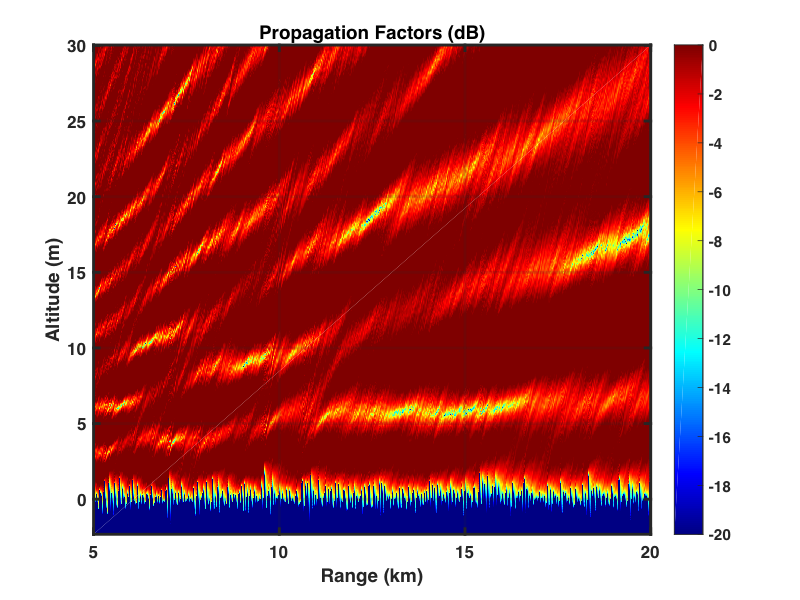
\includegraphics[width=4in]{../media/statistics/pf_1.png}
  \end{center}
  \renewcommand{\baselinestretch}{1} \small\normalsize
  \begin{quote}
    \caption[Example Propagation Factor Realization]{Example Propagation Factor Realization\label{stat_fig:1a}}
  \end{quote}
\end{figure}
\renewcommand{\baselinestretch}{2} \small\normalsize

\begin{figure}[H]
  \begin{center}
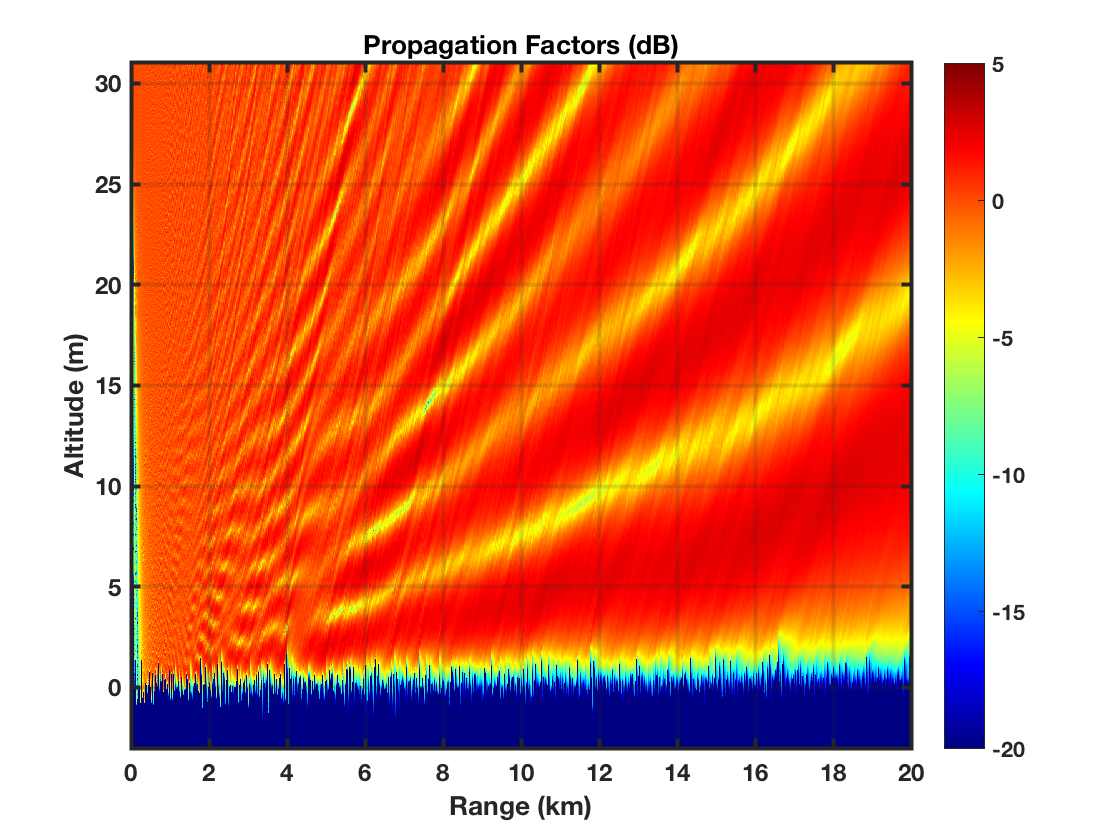
\includegraphics[width=4in]{../media/statistics/pf_2.png}
  \end{center}
  \renewcommand{\baselinestretch}{1} \small\normalsize
  \begin{quote}
    \caption[Example Propagation Factor Realization]{Example Propagation Factor Realization\label{stat_fig:1b}}
  \end{quote}
\end{figure}
\renewcommand{\baselinestretch}{2} \small\normalsize

\subsection{General Monte Carlo Results}
The mean and standard deviation with a 5 m/s wind speed and a $0^\circ$ wind direction are shown in Figure \ref{stat_fig:1zz} for standard atmosphere, and in Figure \ref{stat_fig:1zzz} for a 20 m duct.

\begin{figure}[H]
  \begin{center}
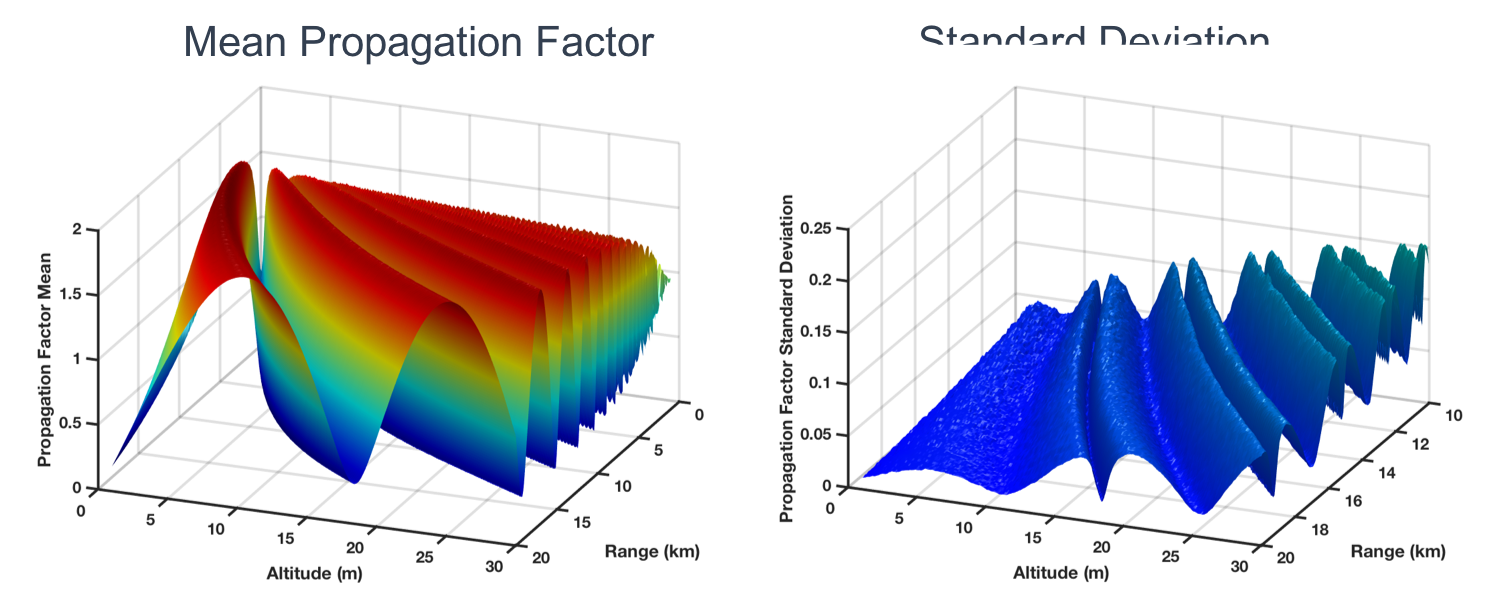
\includegraphics[width=5.5in]{../media/multistatic/std_atmos_results.png}
  \end{center}
  \renewcommand{\baselinestretch}{1} \small\normalsize
  \begin{quote}
    \caption[Standard Atmosphere Statistics at 5 m/s and $0^{\circ}$ Wind]{Standard Atmosphere Statistics at 5 m/s and $0^{\circ}$ Wind\label{stat_fig:1zz}}
  \end{quote}
\end{figure}
\renewcommand{\baselinestretch}{2} \small\normalsize

\begin{figure}[H]
  \begin{center}
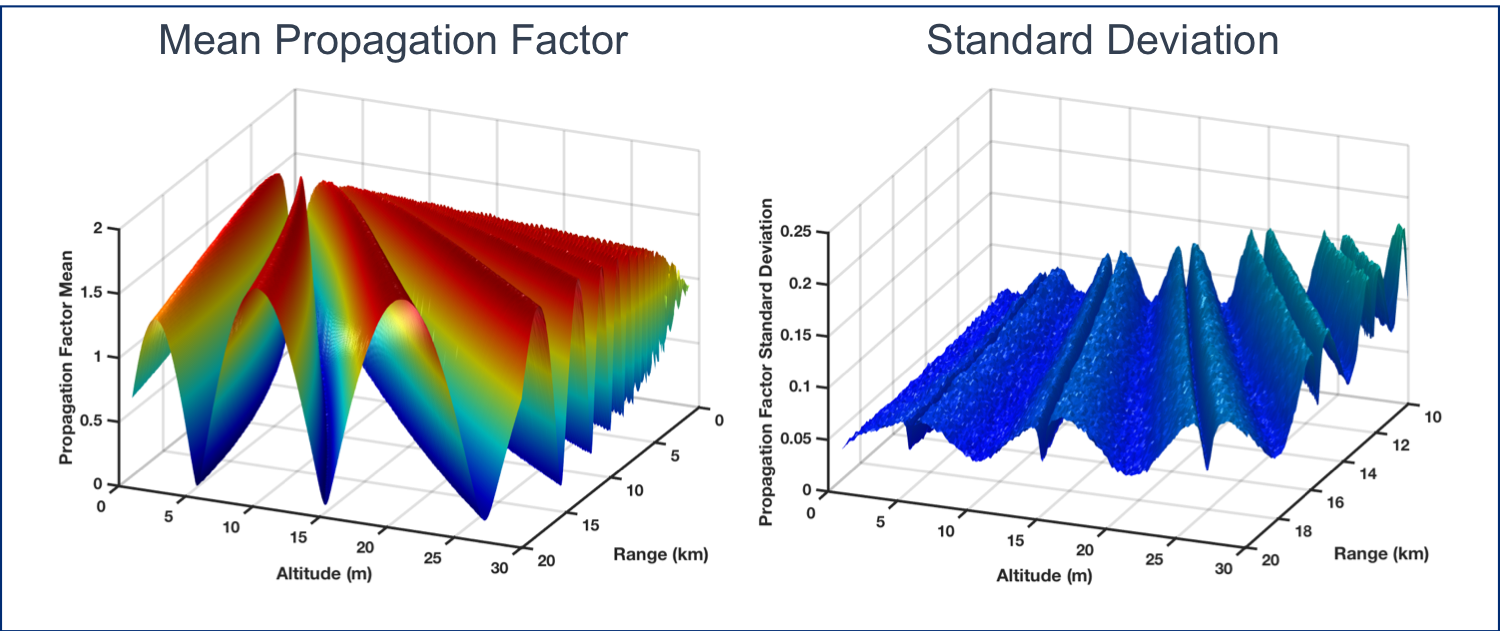
\includegraphics[width=5.5in]{../media/multistatic/duct_results.png}
  \end{center}
  \renewcommand{\baselinestretch}{1} \small\normalsize
  \begin{quote}
    \caption[20 m Duct Statistics at 5 m/s and $0^{\circ}$ Wind]{20 m Duct Statistics at 5 m/s and $0^{\circ}$ Wind\label{stat_fig:1zzz}}
  \end{quote}
\end{figure}
\renewcommand{\baselinestretch}{2} \small\normalsize

In both of these cases, we see that the standard deviation has deep nulls that are co-aligned with nulls in the mean and shallower nulls that are co-aligned with peaks in the mean. These results make sense if we think of propagation of a bundle of rays; at the peaks and nulls in the mean, the rays are all either strongly coherent (peak) or strongly anti-coherent (null). At these extremes, there is little phase variation between the waves and less room for variation in received power. This result also indicates that the standard deviation oscillates at twice the rate of the mean value. 

\subsection{Diffractive Phase Shift}
Figure \ref{stat_fig:2zz} shows the mean propagation factor vs. altitude at a constant range (20 km) for various wind speeds and Figure \ref{stat_fig:2zzz} shows the mean propagation factor vs. altitude at a constant range (20 km) for various wind direction angles. These plots demonstrate there is a diffractive phase shift incurred when propagating over a numerical surface instead of a flat surface with the Miller-Brown approximation.

\begin{figure}[H]
  \begin{center}
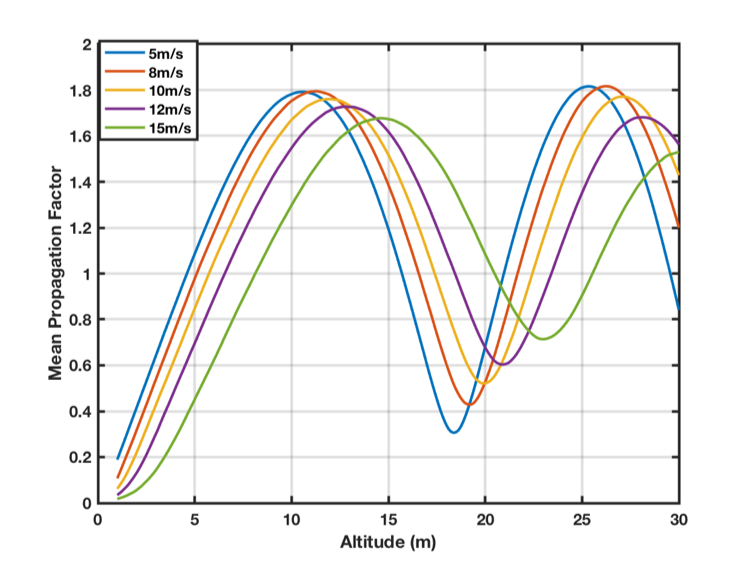
\includegraphics[width=4in]{../media/statistics/phase_shift_wind_speed.png}
  \end{center}
  \renewcommand{\baselinestretch}{1} \small\normalsize
  \begin{quote}
    \caption[Phase Shift at Constant Range due to Wind Speed]{Phase Shift at Constant Range due to Wind Speed\label{stat_fig:2zz}}
  \end{quote}
\end{figure}
\renewcommand{\baselinestretch}{2} \small\normalsize

As shown in Figure \ref{stat_fig:2zz}, increasing the wind speed reduces the amplitude of the mean propagation factor and shifts the phase of the multipath peaks and nulls upward in altitude. The amplitude reduction is expected because higher wind speeds create sea surfaces with more energy which in turn means less RF energy is reflected in the forward direction.

\begin{figure}[H]
  \begin{center}
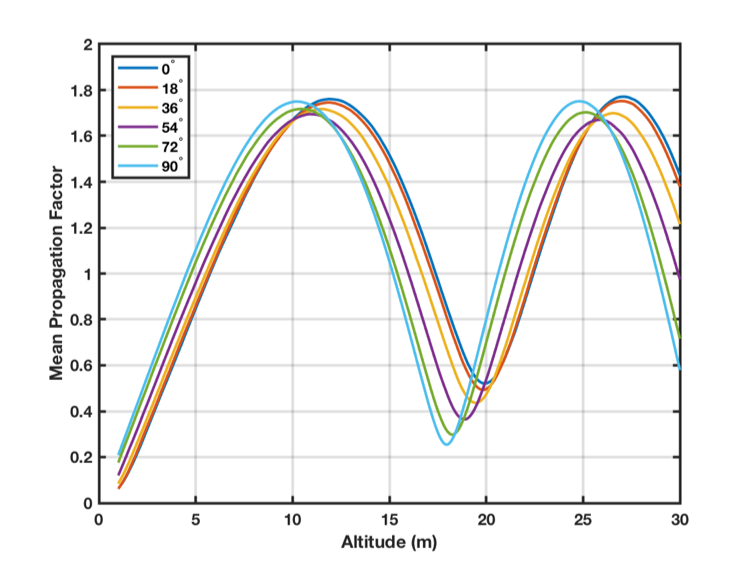
\includegraphics[width=4in]{../media/statistics/phase_shift_wind_direction.png}
  \end{center}
  \renewcommand{\baselinestretch}{1} \small\normalsize
  \begin{quote}
    \caption[Phase Shift at Constant Range due to Wind Direction]{Phase Shift at Constant Range due to Wind Direction\label{stat_fig:2zzz}}
  \end{quote}
\end{figure}
\renewcommand{\baselinestretch}{2} \small\normalsize

As shown in Figure \ref{stat_fig:2zzz}, decreasing the wind direction also shifts the phase of the multipath peaks and nulls upward. In this case, the amplitude does not monotonically decrease because changing the wind direction actually changes the power spectrum surface \cite{frazier_ocean} rather than simply affecting the overall amplitude.

\subsection{PDF Fitting Results}
Propagation over the open ocean should result in a system with fairly high losses, so we expect the PDFs to be normally distributed \cite{yeh_first_principles} \cite{yeh_fading}. 

\subsubsection{Example Fitting Metrics}
Figure \ref{stat_fig:4} shows the propagation factor fit at constant range (20 km) at 10 m and 30 m altitude to demonstrate fitting around both a multipath peak and a multipath null. The standard deviation in both cases shown is identical ($\sigma = 0.176$) and in general is very similar for fits made at a constant range but different altitudes.

\begin{figure}[H]
  \begin{center}
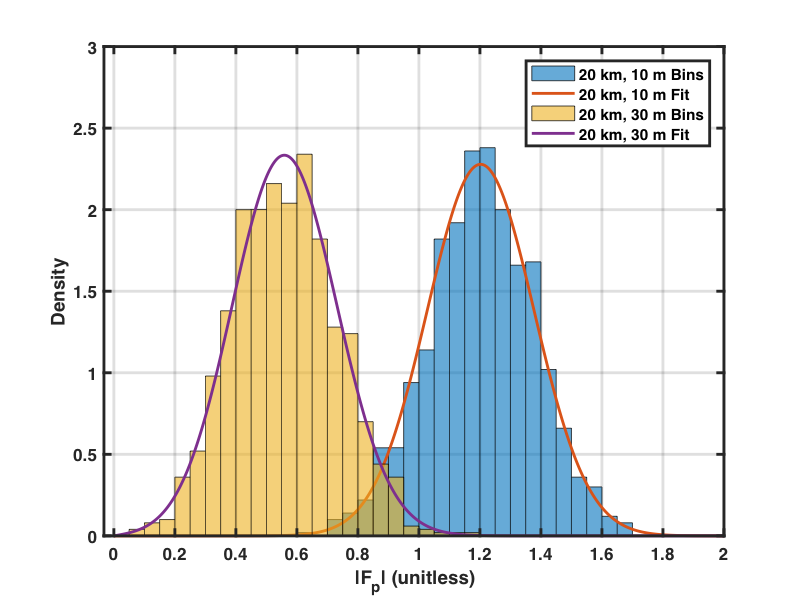
\includegraphics[width=4in]{../media/statistics/constant_range_fit.png}
  \end{center}
  \renewcommand{\baselinestretch}{1} \small\normalsize
  \begin{quote}
    \caption[PDF Fitting at Constant Range]{PDF Fitting at Constant Range\label{stat_fig:4}}
  \end{quote}
\end{figure}
\renewcommand{\baselinestretch}{2} \small\normalsize

Figure \ref{stat_fig:5} shows the propagation factor fit at constant altitude (10 m) at 10 km and 15 km range, again to demonstrate fitting around both a multipath peak and a multipath null. The standard deviation is no longer the same ($\sigma_{10} = 0.223$ while $\sigma_{15} = 0.188$). In general, the standard deviation is not similar for fits made at a constant altitude but different ranges. This indicates range has a stronger impact than altitude.

\begin{figure}[H]
  \begin{center}
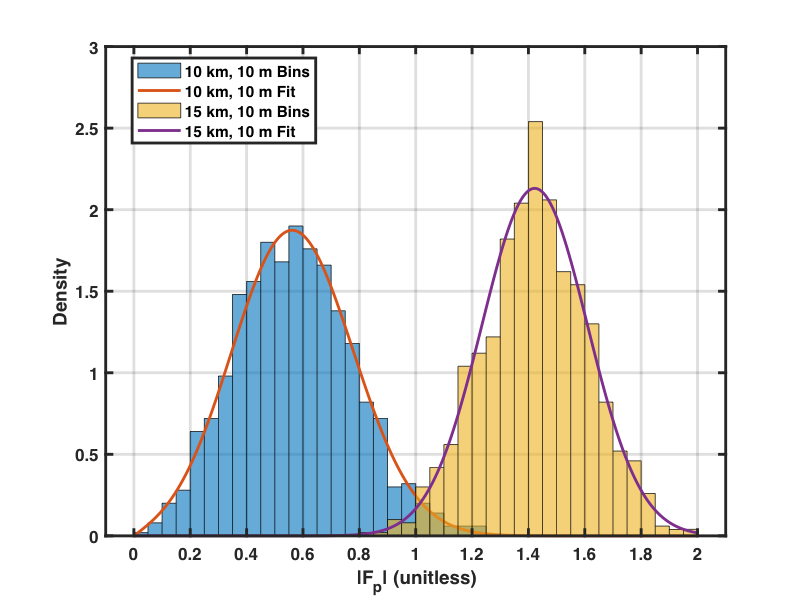
\includegraphics[width=4in]{../media/statistics/constant_altitude_fit.png}
  \end{center}
  \renewcommand{\baselinestretch}{1} \small\normalsize
  \begin{quote}
    \caption[PDF Fitting at Constant Altitude]{PDF Fitting at Constant Altitude\label{stat_fig:5}}
  \end{quote}
\end{figure}
\renewcommand{\baselinestretch}{2} \small\normalsize

\subsection{Loss Parameter Estimation}
As shown in \cite{yeh_fading}, the relationship between the standard deviation, $\sigma$, of the PDF and the loss parameter, $\alpha$, that describes the RMT result is given by

\begin{equation}
\alpha = \frac{1}{\pi\sigma^2}
\end{equation}
\renewcommand{\baselinestretch}{2} \small\normalsize

With this relationship, we can use RMT to match the signal fluctuations around a predetermined average propagation factor.

From \cite{frazier_green}, we can express the phase difference between the primary and the reflected ray as

\begin{equation}
\Delta\phi = 2k\frac{h_1h_2}{L}
\end{equation}
\renewcommand{\baselinestretch}{2} \small\normalsize

Using the observation that the standard deviation oscillates at twice the rate of the mean value, we can break the standard deviation, $\sigma$, into an oscillatory term, $\sigma_s$, and an envelope term $\sigma_d$ so that $\sigma = \sigma_s \sigma_d$. The mean value oscillates relative to $Re\{\exp\left[j\Delta\phi\right]\} = \cos\left(\Delta\phi\right)$. Because the standard deviation must be out of phase with the mean, $\sigma_s$ can be approximated as:

\begin{equation}
\sigma_s = \sin^2\left(2k\frac{h_1h_2}{L}\right)
\end{equation}
\renewcommand{\baselinestretch}{2} \small\normalsize

For a 1-d system, the loss parameter can be approximated as $a \approx kL/Q$, where $Q$ is the quality factor of a given cavity. $Q$ is defined as \cite{pozar_microwave}

\begin{equation}
Q = \omega_0\frac{\text{Energy Stored}}{\text{Power Lost}}
\end{equation}
\renewcommand{\baselinestretch}{2} \small\normalsize

For sufficiently shallow grazing angles there is little backscatter for clutter and we can assume all the energy is either absorbed into the ocean or scattered forward towards the target. Because we are working with propagation factors, we can normalize the transmitted power and approximate an effective quality factor as

\begin{equation}
Q \approx \omega_o\frac{1-\Gamma_t}{\Gamma_t^2}
\end{equation}
\renewcommand{\baselinestretch}{2} \small\normalsize

Here, $\Gamma_t$ is the total reflection coefficient as described in Section \ref{section_reflection_coefficient}, which is dependent on the grazing angle and the RMS ocean wave height, $\sigma_h$.

RMT predicts that the voltage fluctuations will be normally distributed with standard deviation given by $\sigma = \sqrt{(\pi \alpha)^{-1}}$. Since we are looking at fluctuations in power, this standard deviation in voltage will be the variance in power so that

\begin{equation}
\sigma_d = \sqrt{\sigma} = \left( \frac{1}{\pi\alpha} \right)^{1/4}
\end{equation}
\renewcommand{\baselinestretch}{2} \small\normalsize

This assumes that the entire path length, $L$, contributes, so we need to add a scale factor that is the ratio of the region over which the reflected energy is not negligible, $\tilde{x}$ to the total down range distance, $L$. With this scale factor, the envelope term becomes:

\begin{equation}
\sigma_d \approx \frac{1}{4} \left(\frac{1}{\pi \alpha}\right)^{1/4}\left(\frac{\tilde{x}}{L}\right)
\end{equation}
\renewcommand{\baselinestretch}{2} \small\normalsize

\noindent From \cite{frazier_green}, we can express $\tilde{x}$ as:

\begin{equation}
\tilde{x} = \sqrt{\frac{2}{kL_0''}}
\end{equation}
\renewcommand{\baselinestretch}{2} \small\normalsize

\noindent Where $L_0''$ is given as:
\begin{equation}
L_0''=\frac{(h_1+h_2)^4}{h_1h_2L^3} 
\end{equation}
\renewcommand{\baselinestretch}{2} \small\normalsize

\noindent The predicted propagation factor standard deviation is then:
\begin{equation}
\sigma = \sin^2\left(2k\frac{h_1h_2}{L}\right) \frac{1}{4}\left(\frac{\omega_0(1-\Gamma_t)}{\pi kL\Gamma_t^2}\right)^{1/4}\left(\frac{\tilde{x}}{L}\right)
\label{stat_eq:zzz}
\end{equation}
\renewcommand{\baselinestretch}{2} \small\normalsize

Figure \ref{stat_fig:a1} compares the predicted result with the numerical results for 10 mps wind speed at two different wind directions (0 $^{\circ}$ and 36$^{\circ}$). The target point in both cases is at 20 m in altitude.

\begin{figure}[H]
  \begin{center}
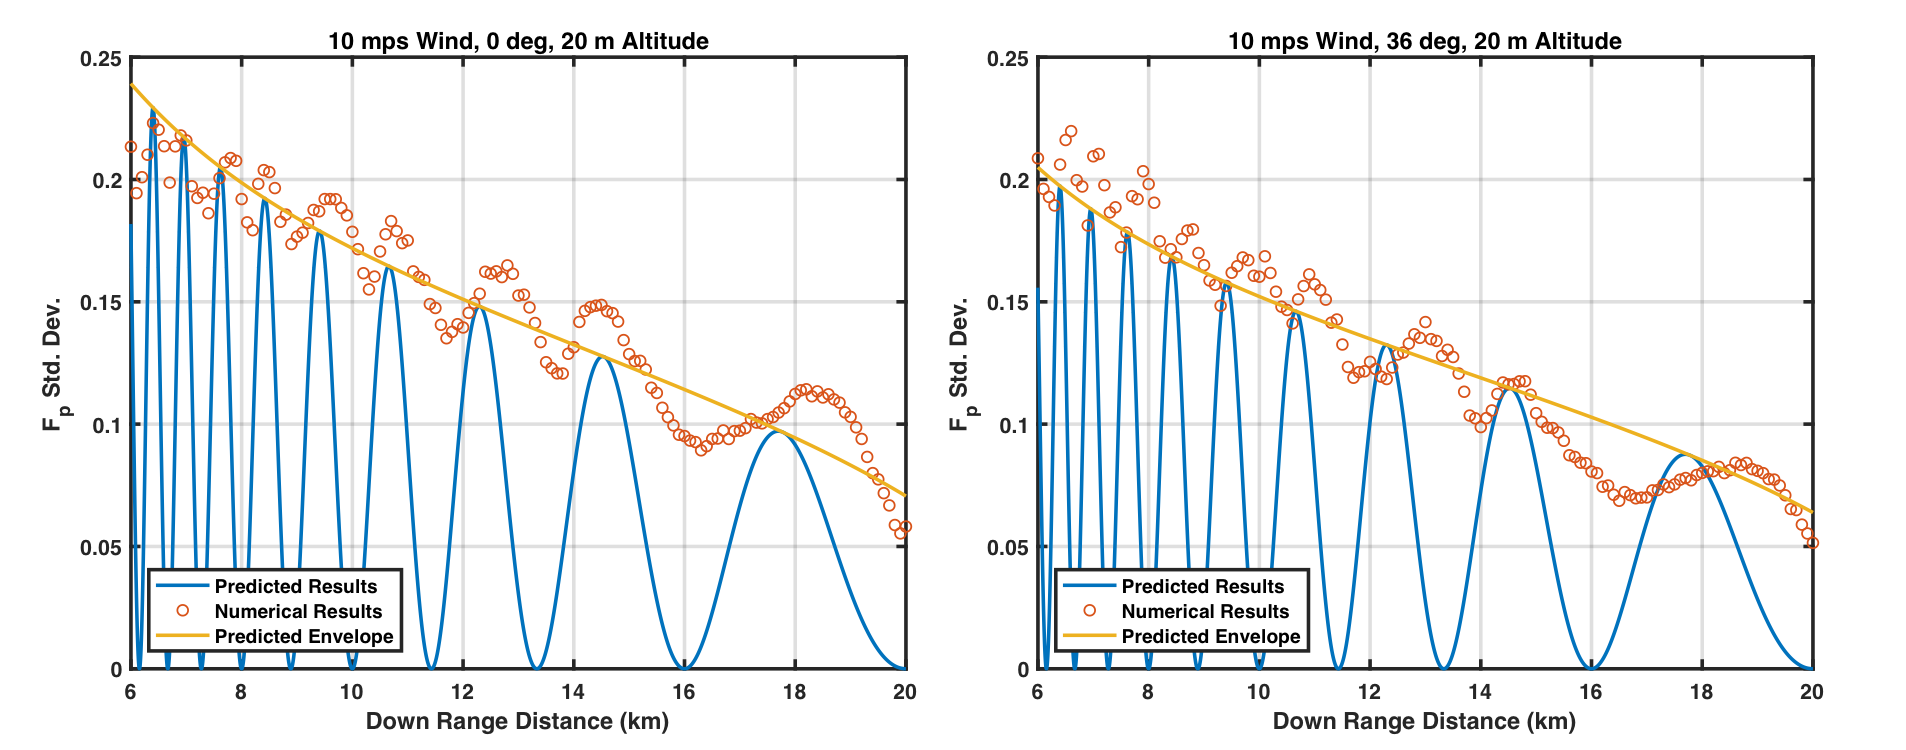
\includegraphics[width=6in]{../media/statistics/predicted_results_wind_direction.png}
  \end{center}
  \renewcommand{\baselinestretch}{1} \small\normalsize
  \begin{quote}
    \caption[$F_p$ Standard Deviation Comparison vs. Wind Direction]{$F_p$ Standard Deviation Comparison vs. Wind Direction\label{stat_fig:a1}}
  \end{quote}
\end{figure}
\renewcommand{\baselinestretch}{2} \small\normalsize

Figure \ref{stat_fig:a1} compares the predicted result with the numerical results directly down range (0$^{\circ}$ wind direction) at two different wind speeds (8 mps and 12 mps). Again, the target point in both cases is at 20 m in altitude.

\begin{figure}[H]
  \begin{center}
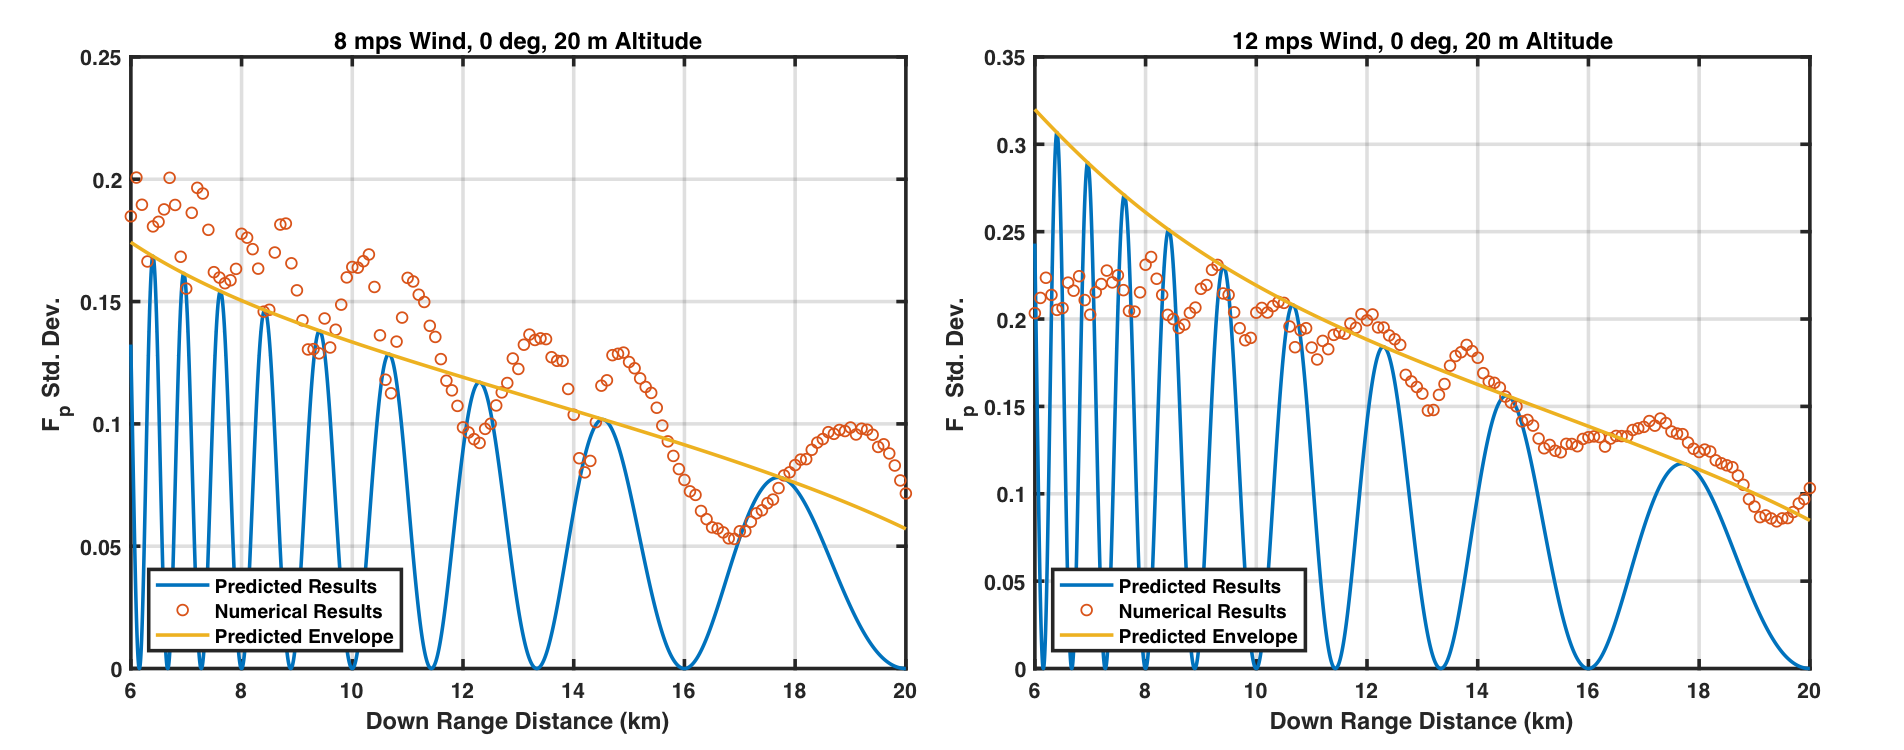
\includegraphics[width=6in]{../media/statistics/predicted_results_wind_speed.png}
  \end{center}
  \renewcommand{\baselinestretch}{1} \small\normalsize
  \begin{quote}
    \caption[$F_p$ Standard Deviation Comparison vs. Wind Speed]{$F_p$ Standard Deviation Comparison vs. Wind Speed\label{stat_fig:a2}}
  \end{quote}
\end{figure}
\renewcommand{\baselinestretch}{2} \small\normalsize 

In both Figure \ref{stat_fig:a1} and Figure \ref{stat_fig:a2}, the envelope term is a good match for the standard deviation when the assumption of shallow grazing angles is valid. As the wind speed increases, this assumption becomes tighter and indicates deviations from the model at short ranges. The location of the peaks and nulls do not line up because the predicted results do not include any corrections for the phase shift. 

Equation \ref {stat_eq:zzz} provides a reasonable approximation for the propagation factor standard deviations shown in Figure \ref{stat_fig:1zz} and Figure \ref{stat_fig:1zzz} but does not include the diffractive phase shift. Using this equation allows us to include propagation factor statistics around a single TEMPER baseline run rather than requiring many iterations. More work is needed to verify this approach over a wider range of conditions and determine the limitations for various geometries.

 \titleformat{\chapter}{\normalfont\bfseries\Large}{Appendix \thechapter}{1em}{}
\appendix
\renewcommand{\thechapter}{A}
\newpage
\appendix
\chapter{Geometric Derivations}

\newpage
\bibliographystyle{unsrt} 
\bibliography{background_bib}

\end{document}












